\documentclass[lettersize,journal]{IEEEtran}
\usepackage{array}
\usepackage[caption=false,font=normalsize,labelfont=sf,textfont=sf]{subfig}
\usepackage{textcomp}
\usepackage{stfloats}
\usepackage{url}
\usepackage{verbatim}
\usepackage{makecell}

% === Chinese support (footnotes only) ========================================
% Works with pdfLaTeX (CJKutf8) and XeLaTeX (xeCJK). XeLaTeX is recommended.
\usepackage{iftex}
\ifPDFTeX
  \usepackage[utf8]{inputenc}
  \usepackage[T1]{fontenc}
  \usepackage{CJKutf8}
  % Chinese-in-footnote helper for pdfLaTeX:
  \newcommand{\cnfn}[1]{\footnote{\begin{CJK*}{UTF8}{gbsn}#1\end{CJK*}}}
\else
  % XeLaTeX/LuaLaTeX: prefer XeLaTeX
  \usepackage{fontspec}
  \ifXeTeX
    \usepackage{xeCJK}
    \setCJKmainfont{Noto Sans CJK SC} % or any installed SC font
    \newcommand{\cnfn}[1]{\footnote{#1}}
  \else
    % LuaLaTeX fallback: luatexja for CJK
    \usepackage{luatexja}
    \newcommand{\cnfn}[1]{\footnote{#1}}
  \fi
\fi
% === End Chinese support ======================================================


\usepackage{amsmath,amssymb,amsfonts}
\usepackage{mathtools}
\usepackage{amsthm}
\usepackage{graphicx}
\usepackage{booktabs}
\usepackage{multirow}
\usepackage{enumitem}
\usepackage{algorithm}
\usepackage{algpseudocode}
\usepackage[table,x11names,dvipsnames]{xcolor}
\usepackage{hyperref}
\hypersetup{hidelinks}
\newcommand{\ci}[2]{#1\,\scriptsize$\pm$\,#2}
\newcommand{\reld}[1]{\textsuperscript{\scriptsize #1}}
\newcommand{\sig}{}
\renewcommand{\arraystretch}{0.99}
% ------- Theorem environments -------
\newtheorem{definition}{Definition}
\newtheorem{theorem}{Theorem}
\newtheorem{proposition}{Proposition}
\newtheorem{assumption}{Assumption}
\newtheorem{lemma}{Lemma}
\newtheorem{remark}{Remark}
\newtheorem{corollary}[theorem]{Corollary}
% helpers for small colored % changes
% ---------- helper macros for table highlights ----------
\newcommand{\best}[1]{\textbf{\underline{#1}}}
\newcommand{\second}[1]{\underline{#1}}
% -------------------------------------------------------


\hyphenation{op-tical net-works semi-conduc-tor IEEE-Xplore}
\def\BibTeX{{\rm B\kern-.05em{\sc i\kern-.025em b}\kern-.08em
    T\kern-.1667em\lower.7ex\hbox{E}\kern-.125emX}}
\usepackage{balance}

\usepackage[markup=underlined]{changes}
\definechangesauthor[name={Me}, color=blue]{me}
\newcommand{\add}[1]{\added[id=]{#1}}

\begin{document}
\begin{CJK*}{UTF8}{gbsn}
\title{Textless, Tiny, and Private: Hashed n\mbox{-}grams with LLM\mbox{-}Teacher Distillation and Local Differential Privacy for Mental\mbox{-}Health Screening on Social Media}
\author{
\IEEEauthorblockN{Dandan Liu\IEEEauthorrefmark{1}, 
Guangrui Fan\IEEEauthorrefmark{2}\thanks{Corresponding author: Guangrui Fan.}, 
Qian Guo\IEEEauthorrefmark{2},
Rui Zhang\IEEEauthorrefmark{2}, and 
Lihu Pan\IEEEauthorrefmark{2}}\\
\IEEEauthorblockA{\IEEEauthorrefmark{1}Faculty of Arts and Social Sciences, 
Universiti Malaya, Kuala Lumpur, Malaysia\\
Email: s2134717@siswa.um.edu.my}\\
\IEEEauthorblockA{\IEEEauthorrefmark{2}School of Computer Science and Technology, 
Taiyuan University of Science and Technology, Taiyuan, China\\
Email: \{fgr, guoqian, zhangrui, panlh\}@tyust.edu.cn}
}
\markboth{IEEE Transactions on Computational Social Systems}%
{Liu \MakeLowercase{\textit{et al.}}: Textless, Tiny, and Private}


\maketitle


\begin{abstract}
We present a textless, compute-light pipeline for user-level mental-health screening on social media that combines salted hashed character $n$-grams, local differential privacy (LDP), and LLM-teacher concept distillation into a tiny, calibrated logistic classifier. The encoder stores no vocabulary or raw text; instead, all posts for a user are aggregated on device into a salted hashed presence vector, and a subsampled randomized-response mechanism is applied once per user to provide an explicit user-level LDP guarantee for this representation. To recover interpretability without online LLMs, we invoke frozen large language models (one for Chinese and one for English) on a small, stratified subset to label clinically grounded concepts (e.g., hopelessness, self-blame, sleep disturbance, help-seeking); compact students are then trained on hashed features to predict these concepts across the full corpus. On two large Weibo user-level corpora, our Hashed\,+\,DP\,+\,Concepts model achieves calibrated utility competitive with a dense-embedding baseline while retaining a CPU-only footprint. Relative to a hashed baseline without concepts, we observe consistent gains in macro-AUPRC and substantially lower calibration error after isotonic mapping. Privacy audits show that, at our default user-level privacy budget, LDP plus salt rotation reduces user-level membership-inference attack success, resists reconstruction compared to embedding inversion, and substantially lowers cross-deployment linkage AUC toward chance in our empirical setting. We release code and audit scripts to facilitate responsible reuse \footnote{https://github.com/GerryFAN0706/Hashed-n-grams-with-LLM-Teacher-Distillation}. 
\end{abstract}



\begin{IEEEkeywords}
mental health, social media, feature hashing, differential privacy, large language models, concept bottlenecks, calibration, membership inference
\end{IEEEkeywords}




% =========================================================
\section{Introduction}
Social platforms provide large-scale traces of language and behavior that can reveal mental-health risk at the user level. Public corpora such as the Reddit Self-reported Depression Diagnosis dataset and the Self-reported Mental Health Diagnoses collection have enabled reproducible research on depression and other conditions in the wild, demonstrating that clinically relevant signals can be detected from naturalistic social-media text \cite{yates2017rsdd,cohan2018smhd}. However, deploying such models in settings like clinics, student services, or NGOs raises two recurring challenges: (i) the need for compute-light methods that can be trained and served on modest hardware; and (ii) the need for privacy-first representations that reduce the risk of exposing sensitive user content.

A growing body of work shows that simple linear models over n\mbox{-}gram features remain strong text-classification baselines while being orders of magnitude more efficient than fine-tuned large models \cite{joulin2017bag}. A key enabler is feature hashing (the ``hashing trick''), which maps high-dimensional n\mbox{-}gram features into a fixed, sparse space with bounded distortion and without storing a vocabulary \cite{weinberger2009featurehashing}. In practice, hashing makes the encoder stateless, memory-light, and fast to train on CPUs, and it is widely available in standard toolkits \cite{scikit2025hashingvectorizer}. These properties make hashed n\mbox{-}grams attractive for mental-health screening pipelines that must be simple to maintain and easy to deploy.

Privacy risks amplify the need to favor such encoders. Dense text embeddings and large language models (LLMs) can reveal information about their training data: attacks have demonstrated membership inference against learned classifiers, as well as training-data extraction of verbatim strings from powerful LLMs \cite{shokri2017mia,shejwalkar2021nlpmia,carlini2021extracting}. For mental-health applications, in which text often contains personal disclosures, minimizing reliance on invertible representations at inference time is prudent. Moreover, recent LLM-based depression detectors highlight strong performance but at significant computational and privacy cost when used online \cite{qin2023readdiagnosechat}. A recurring pitfall in privacy reporting is to rely on empirical membership-inference attack (MIA) metrics as a proxy for privacy guarantees. In this work, MIAs are treated strictly as diagnostics; formal privacy guarantees come from local DP accounting. Concretely, we move randomization to the user level (one-shot per user/window) rather than per post. This collapses naive composition from $B\,r\,\epsilon_b$ (posts $B$, subsample size $r$) to $r\,\epsilon_b$ at the user level, yielding a defensible $\epsilon_{\text{user}}$ without weakening our compute footprint \cite{duchi2013localprivacy,kairouz2015composition,bittau2017prochlo}.

To address these concerns, we adopt local differential privacy (LDP) as the security boundary. Under LDP, randomization occurs on the client side before any data leaves the device, so servers never observe raw text. Mature systems such as RAPPOR and deployments like Apple’s ``Learning with Privacy at Scale'' show that randomized encodings over hashed string features can provide formal guarantees while retaining utility for frequency estimation and monitoring \cite{erling2014rappor,wang2017ldp,apple2017privacy}. This suggests a practical route for privacy-preserving text analytics: combine salted hashing with lightweight randomized response to produce textless features with explicit privacy parameters.

While we avoid heavy training, we still seek interpretability and accuracy. We therefore use LLMs offline as teachers to annotate psychologically meaningful concepts, and then distill these labels into a tiny student that operates purely on hashed features \cite{hinton2015distilling,demszky2020goemotions}. Framing the detector as a concept bottleneck model helps deliver transparent, auditable predictions that can be inspected or intervened upon without exposing raw text \cite{koh2020concept}. In parallel, we calibrate predicted probabilities (e.g., via Platt scaling or isotonic regression) so that downstream screening thresholds can be set responsibly \cite{guo2017calibration,zadrozny2002calibration}.

We present a textless, CPU-trainable pipeline for user-level mental-health screening on social media that combines (1) hashed character $n$-grams with local differential privacy, and (2) LLM-teacher distillation into concept bottlenecks, followed by a small, calibrated logistic classifier. At inference time, the system consumes only hashed features and aggregated concept summaries (no raw text and no LLM). On-device randomization of both the hashed presence vector and the concept summary yields a combined user-level LDP guarantee $\epsilon_{\text{user}} \le 8.8$ under basic composition in our default configuration (formal derivation in Secs.~\ref{sec:ldp}--\ref{sec:boundary}).

Contributions of this paper are:
\begin{enumerate}[label=(\roman*), leftmargin=2em, itemsep=3pt]
\item \textbf{Tiny, deployable encoder with user-level LDP.} We formalize a stateless, textless representation based on salted feature hashing for character $n$-grams and introduce a one-shot user-level local randomizer over the aggregated hashed presence vector $X_u$, satisfying $\epsilon_{\text{hash}}{=}r\,\epsilon_b$-LDP and avoiding the non-defensible $B\,r\,\epsilon_b$ growth of naive per-post schemes \cite{weinberger2009featurehashing,duchi2013localprivacy,kairouz2015composition}.
\item \textbf{Privacy by design; MIAs as diagnostics only.} We report formal local-DP guarantees at the user level and treat membership inference (including LiRA-like attacks) as diagnostic evidence \cite{shokri2017mia,shejwalkar2021nlpmia}. Salt rotation empirically reduces cross-deployment linkage but does not affect the LDP guarantee itself.
\item \textbf{LLM$\rightarrow$tiny concept distillation.} We use frozen LLMs offline to label interpretable concepts and distill them into compact students that operate on hashed features, preserving interpretability without online LLM inference \cite{koh2020concept,hinton2015distilling,demszky2020goemotions}.
\item \textbf{Responsible scoring \& auditing.} We pair calibrated utility with a broadened threat model (white-box MIAs, salt compromise, correlated contributions) and evaluate calibration, privacy, and efficiency side-by-side on user-level mental-health datasets \cite{erling2014rappor,wang2017ldp,acharya2019hr}.
\end{enumerate}




\section{Related Work}
\label{sec:related}

\subsection{Feature hashing for efficient text representations}
The ``hashing trick'' maps sparse n\mbox{-}gram features into a fixed, low-memory space with bounded distortion, enabling fast, stateless encoders that avoid storing vocabularies. Canonical work formalized feature hashing and its theoretical behavior (collision properties, inner‑product preservation) for large‑scale text learning \cite{weinberger2009featurehashing}, and extended the view via hash kernels to connect hashing with kernel approximations on structured inputs \cite{shi2009hashkernels,shi2009hashkernelsjmlr}. Follow‑up analyses relate feature hashing to sparse Johnson–Lindenstrauss embeddings and provide guidance on the number of nonzeros and projection dimension \cite{jagadeesan2019sparsejl}. Classic sketching results (e.g., Count–Min) further contextualize hash‑based counting for high‑cardinality token spaces \cite{cormode2005countmin}. Beyond linear bag‑of‑ngrams, hashing has been used to compress neural layers \cite{chen2015hashednets} and token tables (hash embeddings) \cite{svenstrup2017hashembeddings}, and it is widely deployed in production toolchains such as scikit‑learn and online learners like Vowpal Wabbit \cite{scikit2025hashingvectorizer,vowpalwabbit2018}.  Despite mature theory and wide adoption for efficiency, hashing has not been studied as an explicit privacy mechanism in mental‑health (MH) detection with user‑level privacy audits (e.g., membership inference) or coupled with formal perturbation (DP). To our knowledge, there is no systematic evaluation of hashing + local DP + formal attacks on MH text.

\subsection{Privacy risks in NLP models}
Privacy attacks against text models motivate textless, minimally invertible representations. Membership‑inference attacks (MIAs) were introduced in the black‑box setting and have since been adapted to NLP classifiers, including user‑level audits \cite{shokri2017mia,shejwalkar2021nlpmia}. Modern LLMs can memorize and reveal training data, with empirical demonstrations of unintended memorization and direct extraction of verbatim strings \cite{carlini2019secretsharer,carlini2021extracting,carlini2022memorization}. Even when raw text is not exposed, dense embeddings can leak substantial content via inversion or attribute inference \cite{morris2023vec2text,song2020embeddingsleak,meehan2022sentprivacy}. In collaborative or federated setups, gradients themselves can leak inputs \cite{zhu2019dlg}; recent embedding‑inversion pipelines further reduce the barrier to text reconstruction from sentence representations \cite{li2023geninv}. MH detection papers rarely co‑report utility with privacy metrics (e.g., MIA AUC) and inversion success side‑by‑side. A comparative privacy audit for deployable baselines is missing.

Beyond early confidence-based MIAs, stronger attacks have emerged. LiRA-style attacks compare a target's loss against a shadow distribution to approximate the likelihood ratio, often boosting separability at low FPRs; white-box access further strengthens MIAs by leveraging logits, margins, or gradients \cite{shokri2017mia,shejwalkar2021nlpmia}. Recent work shows that even in-context learning with LLMs is vulnerable to membership inference \cite{wen2024miaicl}. Accordingly, our audits include (i) loss-threshold and LiRA-like MIAs, (ii) black- and white-box settings, and (iii) calibration-aware MIAs that exploit miscalibration.


\subsection{Local differential privacy (LDP) for string/frequency data}
LDP provides client-side randomization so that raw strings or counts are never observed by the server. Practical systems such as RAPPOR \cite{erling2014rappor} established deployability at scale; OLH/OUE \cite{wang2017ldp} and Hadamard Response \cite{acharya2019hr} improved utility for high-cardinality frequency estimation. Foundational results characterize minimax rates and composition under local privacy \cite{duchi2013localprivacy,kairouz2015composition}, and large-scale deployments (Apple's telemetry \cite{apple2017privacy}, Prochlo's Encode--Shuffle--Analyze \cite{bittau2017prochlo}) demonstrate operational feasibility. Recent theory formalizes user-level LDP when each user contributes multiple items, directly relevant to user-centric MH detection \cite{acharya2023userldp}; surveys synthesize the design space \cite{wang2020surveyldp,qin2023ldpsurvey}. Complementary approaches apply local DP to full-text rewriting via generative models \cite{igamberdiev2023dpbart} or LLM-based privatization \cite{meisenbacher2024dpbox}; in contrast, our pipeline avoids retaining text entirely. Adding an anonymizing shuffler can amplify local guarantees; we derive optional amplified accounting (Sec.~\ref{sec:ldp}) and show that tighter local budgets ($\epsilon_{\text{user}} \le 4$) yield strong central guarantees ($\epsilon_c < 1.1$) after shuffling \cite{balle2019shuffle,erlingsson2019shuffle}.

\subsection{Federated learning (FL) for depression detection}
FL has been explored for MH with text and speech, often with deep models and nontrivial system complexity. Studies report FL for multilingual depression detection with transformer encoders \cite{khalil2024patterns}, smartphone/on‑device FL using social‑media text \cite{ahmed2024smartphonefl}, and multimodal mobile inputs (keyboard, speech) \cite{shin2023fedtherapist}. Speech‑based depression FL has also been investigated, showing feasibility but still requiring model/infra sophistication \cite{suhas2022flspeech,cui2022flspeechdepression}. Methodological work tackles communication and heterogeneity (e.g., asynchronous FL) in this application \cite{li2022cafed}. Recent surveys position MH FL as emergent and open on evaluation and privacy auditing \cite{grataloup2024surveyflmh}. Newer combinations (e.g., LoRA‑augmented FL) further raise engineering and resource barriers \cite{sarwar2025fedmentalcare}. FL research in MH rarely includes formal privacy audits (e.g., MIA AUC, reconstruction tests) and introduces substantial deployment overhead. A strong, CPU‑trainable, non‑FL baseline with measured privacy remains missing.

\subsection{LLMs for annotation/teacher–student, and concept supervision in MH}
LLMs can act as high‑quality annotators and teachers, enabling low‑cost label generation and model compression without serving LLMs at inference \cite{gilardi2023chatgptannotators,tan2024llmannotationSurvey,hinton2015distilling}. In parallel, concept bottleneck models make intermediate predictors explicit and editable, supporting transparency for sensitive applications \cite{koh2020concept}. Within MH, LLMs have been explored for interpretable analysis and end‑to‑end detection, often relying on online prompting or heavy models \cite{yang2023interpretablellm,qin2023readdiagnosechat}. Distillation techniques tailored to LLM teachers demonstrate that compact students can retain much of the teacher signal \cite{dipalo2024pgkd}. For concept ontologies, fine‑grained emotion taxonomies on Reddit (e.g., GoEmotions) offer a practical scaffold for defining psychologically meaningful targets to distill \cite{demszky2020goemotions}. Domain surveys contextualize clinical opportunities and caveats for LLMs in psychiatry and MH tasks \cite{liu2024llmpsychiatry,xu2025benchmarkmhllm}. Prior MH work seldom combines LLM‑offline annotation (teacher) with a tiny concept‑bottleneck student that runs on textless hashed features under local DP, alongside explicit privacy audits. 

\underline{We bring these threads together}: (i) a stateless, hashed character n\mbox{-}gram encoder with local DP randomization; (ii) an LLM‑teacher that labels interpretable concepts only offline, distilled into a calibrated linear student; and (iii) a joint evaluation that reports utility on public MH datasets together with privacy metrics (membership inference, reconstruction baselines), addressing the gaps identified above.


\section{Method}
\label{sec:method}

\subsection{Problem Setup and Notation}
We consider a set of users $\mathcal{U}$. Each user $u \in \mathcal{U}$ produces a time‑ordered sequence of posts $X_u = \{x_{u,1}, x_{u,2}, \dots, x_{u,T_u}\}$ with timestamps $\{t_{u,1}, \dots, t_{u,T_u}\}$.
The task is user‑level risk prediction: learn a function
\begin{equation}
    f_\theta: \mathcal{X}^{*} \rightarrow [0,1], \qquad \hat{p}_u = f_\theta(X_u),
\end{equation}
that outputs a calibrated probability $\hat{p}_u$ of belonging to the positive class (e.g., exhibiting depression‑related risk), given all available text for $u$.
To meet privacy and compute constraints, we design $f_\theta$ with: (i) feature hashing over character $n$‑grams (textless, vocabulary‑free), (ii) a compact, interpretable concept bottleneck distilled from a frozen large language model (LLM) teacher, and (iii) a local differential privacy (LDP) mechanism that is applied once per user to the aggregated hashed representation and concept summary.

\begin{figure*}[t]
\centering
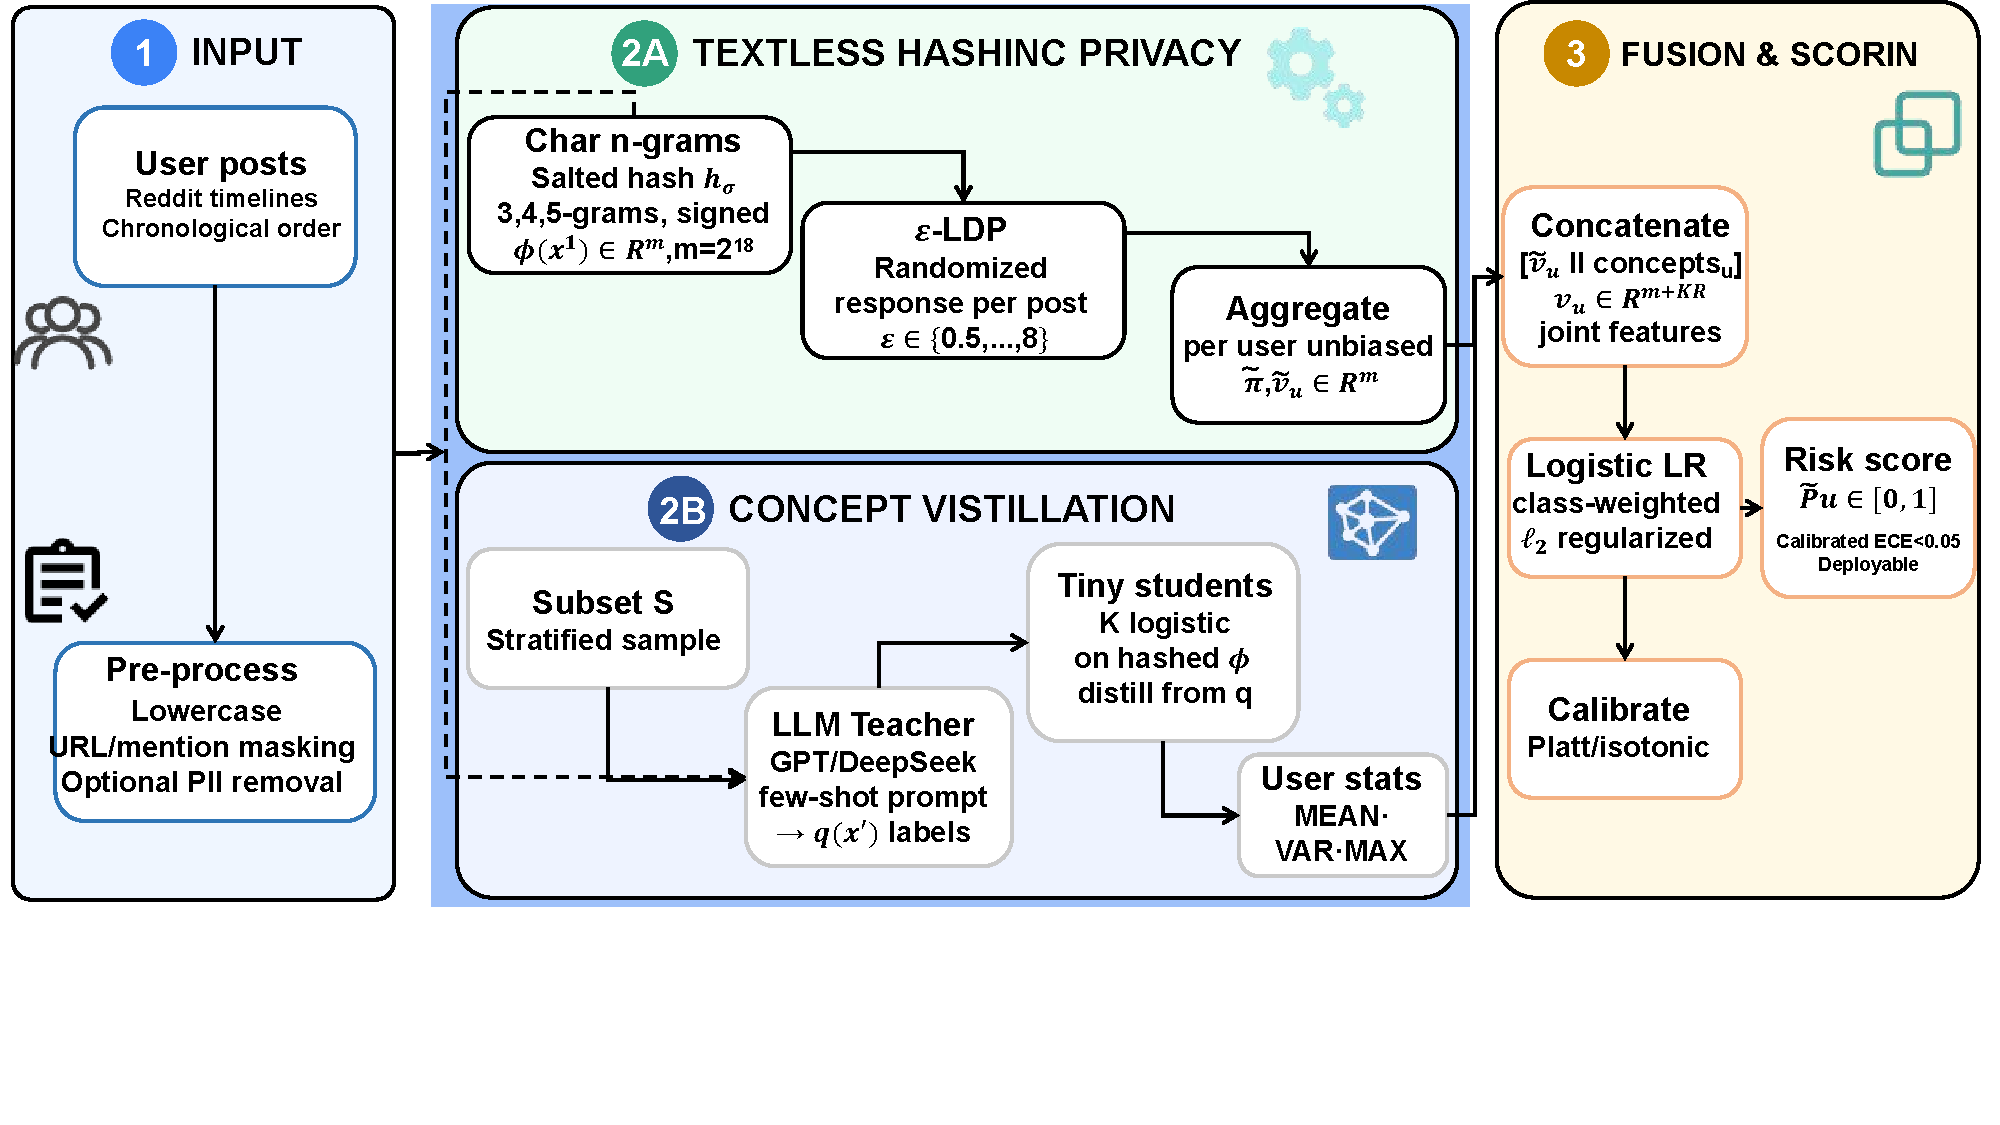
\includegraphics[width=\linewidth]{results_figures/Overview.pdf}
\caption{System overview. All arrows are solid and denote on-device data flow (sanitization $\rightarrow$ hashed/concept features $\rightarrow$ local randomizer $\rightarrow$ server). The \emph{dashed boundaries} around modules 2A (Textless Hashing Privacy) and 2B (Concept Distillation) are stylistic only --- they group the privacy/distillation core for visual readability and do not represent a feedback loop, an optional path, or any data flow. No raw text or LLM call ever crosses the client--server boundary at inference.}
\label{fig:overview}
\end{figure*}

\subsection{Pre‑processing and Optional De‑identification}
Each post $x$ undergoes normalization $g(\cdot)$ (lowercasing, URL/user‑mention masking, whitespace canonicalization) and an optional on‑device de‑identification transform $r(\cdot)$ that replaces personally identifying strings (names, emails, phone numbers, locations) with category placeholders.
We denote the sanitized text by $x' = r(g(x))$ and proceed only with $x'$.
De‑identification reduces obvious re‑identification risk but is not a substitute for formal privacy mechanisms; hence the local DP layer introduced below.

\subsection{Textless Representation via Feature Hashing}
Let $\mathcal{G}(x')$ be the multiset of character $n$‑grams extracted from $x'$ for $n \in \{3,4,5\}$.
We use a pair of hash functions: an index hash $h: \mathcal{G} \to [m]$ and a sign hash $\xi: \mathcal{G} \to \{-1,+1\}$.
The hashed post vector $\phi(x') \in \mathbb{R}^{m}$ is defined component‑wise as
\begin{equation}
    \phi_j(x') \;=\; \sum_{g \in \mathcal{G}(x')} \mathbb{I}\{h(g)=j\}\,\xi(g),
    \quad j \in [m].
\end{equation}
At user level, we form an (unprivatized) hashed summary by additive aggregation
\begin{equation}
    z_u \;=\; \sum_{t=1}^{T_u} \phi(x'_{u,t}) \in \mathbb{R}^{m}.
\end{equation}
To improve privacy, we do not retain $\mathcal{G}$ or any vocabulary; only the fixed $m$‑dimensional hashed vectors are handled downstream. Section~\ref{sec:ldp} introduces a local DP randomizer that acts on the aggregated user‑level vector $X_u$, so that randomization occurs once per user/window rather than per post. Unless otherwise stated, $h(\cdot)$ and $\xi(\cdot)$ are 64‑bit MurmurHash3 keyed by the salt $\sigma$, with a single index hash and a sign hash \cite{weinberger2009featurehashing}. We aggregate signed counts and subsequently binarize per coordinate before privatization (Sec.~\ref{sec:ldp}). Empirically, we found sublinear TF (e.g., $\log(1+\mathrm{count})$) unnecessary once binarization+LDP are applied; when used, we clip per‑post contributions to $[-c_{\max},c_{\max}]$ with $c_{\max}=3$.

\subsection{Concept Bottlenecks via LLM‑Teacher Distillation}
\label{sec:concept}
We define a compact set of psychologically meaningful concepts $\mathcal{C}=\{c_1,\dots,c_{K}\}$ (e.g., cognitive distortions such as catastrophizing, all‑or‑nothing thinking, self‑blame; and clinically relevant states such as hopelessness or help‑seeking).

\paragraph{Psychological grounding of the concept set.}
The inventory $\mathcal{C}$ is constructed with reference to established constructs in cognitive–behavioural theory and depression assessment. Cognitive distortions such as catastrophizing and all‑or‑nothing thinking are central in Beck's cognitive model of depression and cognitive‑behavioural therapy manuals \cite{beck1991cognitive,beck1972measuring}, while hopelessness and anhedonia are core symptom dimensions in widely used scales such as the PHQ‑9 \cite{kroenke2001phq}. Help‑seeking, self‑blame, and social withdrawal are likewise grounded in the clinical literature on coping, interpersonal functioning, and risk trajectories in depression. Our goal is not to re‑invent clinical nosology, but to select a small set of interpretable constructs that (i) can be reliably recognized by LLM teachers in short posts, and (ii) are meaningful to clinicians and support staff when presented as model explanations.

\paragraph{Cross-cultural considerations.}
Several of these constructs have demonstrated cross-cultural stability in validation studies of the PHQ-9 and BDI across diverse populations, including Chinese samples \cite{kroenke2001phq,beck1972measuring}: hopelessness, anhedonia, sleep disturbance, and fatigue show consistent factor loadings across Western and East Asian cohorts. Other constructs may manifest differently: self-blame in collectivist cultures can co-occur with relational guilt rather than purely individual attribution, and help-seeking is subject to stronger stigma effects on Chinese social media \cite{koh2020concept}. We do not yet have bilingual-clinician validation of the concept inventory; the Appendix reports cross-teacher consistency (Pearson $r{=}0.78$ mean across concepts), which is a teacher-\emph{stability} metric rather than clinical validity. Accordingly we position the system as a research-grade screening prototype, not a clinical instrument; expert review across languages is a prerequisite for deployment readiness.
\begin{table}[t]
\centering
\caption{Concept inventory ($K{=}12$) with psychological grounding.}
\label{tab:concepts}
\renewcommand{\arraystretch}{1.05}
\resizebox{\linewidth}{!}{%
\begin{tabular}{p{2.2cm}p{3cm}p{5cm}}
\toprule
\textbf{Concept} & \textbf{Psychological source} & \textbf{Operational definition} \\
\midrule
Hopelessness & PHQ-9, Beck Depression Inventory & Expressing lack of optimism or belief that future will improve \\
Anhedonia & PHQ-9, DSM-5 criteria & Loss of interest or pleasure in previously enjoyed activities \\
Sleep disturbance & PHQ-9 & Reporting insomnia, hypersomnia, or poor sleep quality \\
Appetite/weight & PHQ-9 & Reporting appetite or weight change \\
Fatigue/low energy & PHQ-9 & Expressing low energy, tiredness, or physical exhaustion \\
Concentration diff. & PHQ-9, cognitive assessment & Trouble focusing, indecision, or cognitive slowing \\
Psychomotor change & PHQ-9, clinical observation & Observable agitation or psychomotor retardation cues \\
Self-blame/guilt & Coping \& attribution theory & Attributing negative events to personal failures; excessive guilt \\
Catastrophizing & Beck's cognitive distortions & Exaggerating negative outcomes or believing worst-case scenarios \\
All-or-nothing & Beck's cognitive distortions & Viewing situations in extreme, binary terms without middle ground \\
Social withdrawal & Interpersonal theory of depression & Expressing desire to avoid social contact or isolation \\
Help-seeking & Health behavior models & Expressing intent or behavior to seek support or professional help \\
\bottomrule
\end{tabular}
}
\end{table}
A frozen LLM teacher $T$ maps a post to a multi‑label concept distribution:
\begin{equation}
    T: x' \mapsto q(x') \in [0,1]^K, \qquad q_c(x') = \Pr(c \mid x') \;\; \text{for } c \in \mathcal{C}.
\end{equation}
To constrain cost and avoid heavy training, the teacher is invoked only on a small stratified subset $\mathcal{S}$ of posts drawn from the training split; no validation or test data is seen by the teacher, and no user-level depression risk labels are provided to the teacher (only the raw post text). The teacher produces concept probabilities in an unsupervised manner relative to the downstream task. 

\paragraph{Student predictors.}
For each concept $c \in \mathcal{C}$, we train a compact student predictor $s_c(\cdot)$ that consumes only hashed features:
\begin{equation}
    \hat{q}_c(x') \;=\; \sigma\!\left(\frac{\mathbf{w}_c^\top \phi(x') + b_c}{\tau}\right),
\end{equation}
where $\sigma$ is the logistic sigmoid, $\tau>0$ is a temperature, and $(\mathbf{w}_c,b_c)$ are learned via distillation on $\mathcal{S}$ using a proper scoring rule (binary cross‑entropy or KL):
\begin{equation}
    \mathcal{L}_{\text{distill}} 
    \;=\; \sum_{x' \in \mathcal{S}} \sum_{c \in \mathcal{C}} 
    \mathrm{BCE}\!\left(\hat{q}_c(x'),\, q_c(x')\right) \;+\; \lambda \sum_{c}\lVert \mathbf{w}_c \rVert_2^2 .
\end{equation}
After training, $T$ and any raw teacher outputs are discarded; inference uses only $s_c(\cdot)$.

\paragraph{User‑level concept features.}
Student post‑level outputs are aggregated into a per‑user concept feature vector $s_u \in \mathbb{R}^{K \times R}$ via summary operators $\mathcal{A}_r$ (e.g., mean, variance, max, temporal persistence):
\begin{equation}
    s_u \;=\; \bigoplus_{c \in \mathcal{C}} \bigoplus_{r=1}^{R} \mathcal{A}_r\!\left(\{\hat{q}_c(x'_{u,t})\}_{t=1}^{T_u}\right),
\end{equation}
where $\oplus$ denotes concatenation. 
Temporal statistics may include run‑lengths or lag‑1 autocorrelation of concept probabilities to capture persistence without training sequence models.

\begin{figure*}[t]
\centering
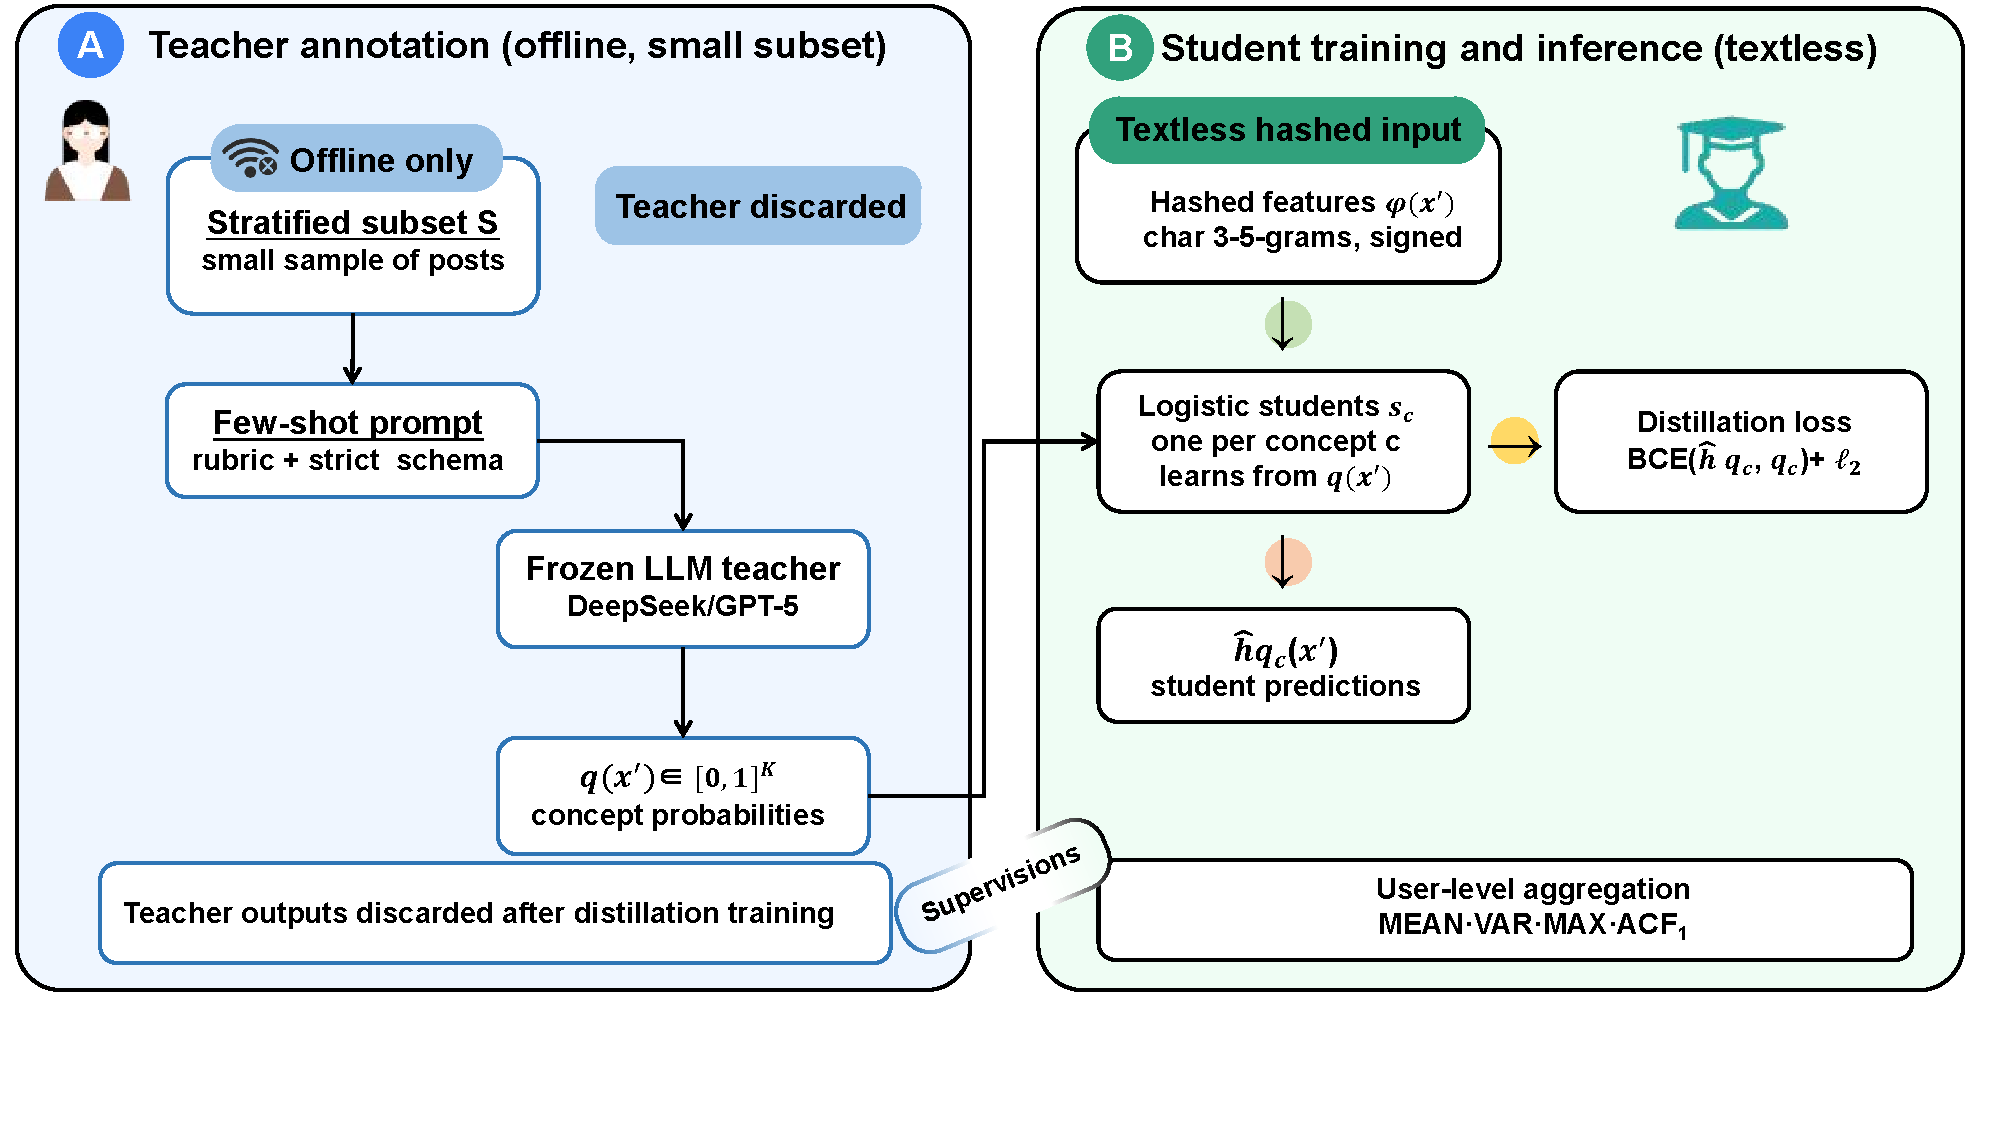
\includegraphics[width=\linewidth]{results_figures/Distillation.pdf}
\caption{Concept bottlenecks distilled from a frozen LLM teacher into tiny hashed‑feature students.}
\label{fig:concept}
\end{figure*}
\paragraph{Aggregation operators.}
Let $\{q_{t,c}\}_{t=1}^{T_u}$ denote the student probabilities for concept $c$ on user $u$'s posts, and $\bar{q}_c=\frac{1}{T_u}\sum_{t} q_{t,c}$. We instantiate $\mathcal{A}_r$ as:
\begin{align}
\mathrm{mean}_c(u) &= \bar{q}_c, \\[4pt]
\mathrm{var}_c(u)  &= \frac{1}{T_u}\sum\nolimits_{t}(q_{t,c}-\bar{q}_c)^2, \\[4pt]
\mathrm{max}_c(u)  &= \max\nolimits_{t}\; q_{t,c}, \\[4pt]
\mathrm{acf1}_c(u) &= \frac{\displaystyle\sum_{t=2}^{T_u}(q_{t,c}-\bar{q}_c)(q_{t-1,c}-\bar{q}_c)}{\displaystyle\sum_{t=1}^{T_u}(q_{t,c}-\bar{q}_c)^2+\delta},
\end{align}
with $\delta=10^{-8}$ for numerical stability. When used, a persistence statistic is
\begin{equation}
\mathrm{max\_run}_c(u)=\max_{t}\Bigl\{\sum\nolimits_{k\ge 0}\mathbb{I}\big[q_{t+k,c}\ge \tau_c\big]\Bigr\},
\end{equation}
with fixed threshold $\tau_c\in[0,1]$ (we use $\tau_c=0.7$ in ablations).

\paragraph{Distillation hygiene.}
We fix temperature $\tau=1.0$ and optionally apply label smoothing on teacher outputs with $\alpha{=}0.05$ (ablation shows negligible effect). Teachers are never invoked at inference; only compact students $s_c(\cdot)$ are used on hashed features.

\subsection{Client--Server Boundary and Concept Feature Privacy}
\label{sec:boundary}

We make the client--server split explicit, since it determines what is protected by local DP.

\paragraph{On-device computations.}
For a given user $u$, all raw posts $\{x_{u,t}\}$ are processed only on the client:
\begin{enumerate}[leftmargin=1.5em,itemsep=2pt]
  \item sanitize and optionally de-identify $x_{u,t}$ to obtain $x'_{u,t}$;
  \item map each $x'_{u,t}$ to a hashed feature vector $\phi(x'_{u,t}) \in \mathbb{R}^m$ as in Sec.~\ref{sec:method};
  \item aggregate across posts into a binarized presence vector
  \begin{equation}
    X_u[j] \;=\; \mathbb{I}\Bigl[\exists t:\,\phi_j(x'_{u,t}) \neq 0\Bigr] \in \{0,1\},
    \quad j \in [m];
  \end{equation}
  \item evaluate the concept students $s_c(\cdot)$ on each post and summarize them into bounded user-level concept features $s_u \in [0,1]^{K\times R}$ as in Sec.~\ref{sec:concept}.
\end{enumerate}

The client then applies two independent local randomizers:
\begin{itemize}[leftmargin=1.4em]
  \item a subsampled randomized-response mechanism $\mathcal{R}_{\text{hash}}$ to $X_u$ (Sec.~\ref{sec:ldp}), producing a length-$r$ bit vector $Y^{\text{hash}}_u$; and
  \item a $G$-ary randomized-response mechanism $\mathcal{R}_{\text{concept}}$ to each scalar entry of $s_u$ (this subsection), producing a discretized, privatized concept summary $\hat{s}_u$.
\end{itemize}
Only the pair $\bigl(Y^{\text{hash}}_u,\hat{s}_u\bigr)$ leaves the device; the server never sees raw text, unhashed features, or non-privatized concept scores.

\paragraph{User-level concept summaries and local privatization.}
Each scalar component of $s_u$ is first rescaled to $[0,1]$ (variance and $\mathrm{acf1}$ are linearly mapped to $[0,1]$ as described earlier) and then quantized into $G$ bins. Let $L = K \times R$ be the number of summary statistics per user, and denote the (integer) bin index of the $\ell$-th scalar by $b_{u,\ell} \in \{1,\dots,G\}$. We apply $G$-ary randomized response (KRR) with privacy parameter $\epsilon_c$ to each $b_{u,\ell}$ independently:
\begin{equation}
  \Pr[\hat{b}_{u,\ell} = j \mid b_{u,\ell}]
  = \begin{cases}
      p_c = \dfrac{e^{\epsilon_c}}{e^{\epsilon_c} + G - 1}, & j = b_{u,\ell},\\[0.6ex]
      q_c = \dfrac{1}{e^{\epsilon_c} + G - 1}, & j \neq b_{u,\ell}.
    \end{cases}
\end{equation}
The locally privatized concept report is the vector
$\hat{s}_u = (\hat{b}_{u,1},\dots,\hat{b}_{u,L})$ sent once per user (or per fixed time window). On the server, we apply the standard unbiased KRR de-biasing to recover an estimate $\tilde{s}_u \in [0,1]^L$.

By sequential composition of LDP mechanisms, $\mathcal{R}_{\text{concept}}$ satisfies $L\epsilon_c$-LDP at the user level: the $L$ coordinates are independent and each is $\epsilon_c$-LDP, so the joint mechanism is $(L\epsilon_c)$-LDP. In our default configuration $K{=}12$, $R{=}4$, $G{=}64$, and $\epsilon_c{=}0.05$, hence $L{=}48$ and the concept channel contributes at most
\begin{equation}
  \epsilon_{\text{concept}} \;\le\; L \epsilon_c \;=\; 2.4.
\end{equation}
This bound is intentionally conservative. A R\'enyi-DP analysis at $(\alpha,\delta){=}(8,10^{-6})$ tightens the joint user-level budget from $8.8$ to $\epsilon_{\text{user}}^{\text{RDP}}{\approx}4.3$ ($\sim\!2{\times}$ improvement), with the hashed channel dominating; full derivation and table in the Appendix (Sec.~C, ``Tighter accounting via RDP''). We retain $r\epsilon_b{+}L\epsilon_c$ in the main text as a parameter-free upper bound suitable for privacy cards.



\subsection{User-Level Local Differential Privacy for Hashed Features}
\label{sec:ldp}

We now formalize the subsampled randomized-response mechanism applied to the hashed presence vector $X_u$ and its user-level LDP guarantee.

\begin{definition}[User-level adjacency and LDP]
\label{def:uldp}
Let $X_u \in \{0,1\}^m$ denote the (binarized) hashed feature vector summarizing all posts for user $u$ within a fixed time window. Two inputs $X_u$ and $X_u'$ are adjacent if they correspond to two possible worlds that differ in all contributions of that user in the window (e.g., $X_u'$ is the counterfactual in which the user never posted). A randomized mechanism $\mathcal{M}$ mapping $X_u$ to an output in some space $\mathcal{Y}$ is said to satisfy $\epsilon$-local differential privacy (LDP) at the user level if, for all adjacent $X_u,X_u'$ and all measurable $S \subseteq \mathcal{Y}$,
\begin{equation}
  \Pr[\mathcal{M}(X_u) \in S]
  \;\le\; e^\epsilon \Pr[\mathcal{M}(X_u') \in S].
\end{equation}
\end{definition}

\paragraph{Subsampled randomized response (ULDP-SSR).}
For each user $u$, the client holds $X_u \in \{0,1\}^m$ as defined in Sec.~\ref{sec:boundary}. Using public randomness (a PRF shared with the server), we draw a content-independent index set $R_u \subset [m]$ of fixed size $r \ll m$. Conditioned on $R_u$, we apply independent randomized response with parameter $\epsilon_b$ to each selected bit:
\begin{equation}
  Y_{u,j} \;=\;
  \begin{cases}
    X_{u,j},      & \text{w.p. } p_b,\\[0.8ex]
    1 - X_{u,j},  & \text{w.p. } 1-p_b,
  \end{cases}
  \quad
  p_b = \frac{e^{\epsilon_b}}{1+e^{\epsilon_b}},\;\; j \in R_u.
\end{equation}
The report sent to the server is the length-$r$ vector
$Y^{\text{hash}}_u = (Y_{u,j})_{j \in R_u}$ in the fixed order of $R_u$; the server reconstructs $R_u$ from the public seed and never sees $X_u$ itself.

\begin{proposition}[User-level LDP for ULDP-SSR]
\label{prop:uldp-ssr}
Conditioned on the public randomness used to draw $R_u$, the mechanism $X_u \mapsto Y^{\text{hash}}_u$ described above satisfies $\epsilon_{\text{hash}}$-LDP at the user level with
\begin{equation}
  \epsilon_{\text{hash}} \;=\; r \epsilon_b.
\end{equation}
\end{proposition}

\begin{proof}[Sketch]
Given a fixed index set $R_u$ of size $r$, the mechanism factorizes across coordinates:
\(
  \Pr[Y^{\text{hash}}_u \mid X_u]
  = \prod_{j \in R_u} \Pr[Y_{u,j} \mid X_{u,j}].
\)
Each coordinate is an independent $\epsilon_b$-LDP randomized-response bit, so the likelihood ratio between any two inputs $X_u$ and $X_u'$ is bounded by $e^{r\epsilon_b}$. Taking expectation over the public randomness (choice of $R_u$) preserves this bound by standard convexity arguments in LDP composition \cite{duchi2013localprivacy,kairouz2015composition}.
\end{proof}

\paragraph{Server-side de-biasing.}
On the server side, we obtain an estimate of the hashed presence vector by inverting the RR channel on the observed bits. Let
\[
  \hat{\pi}_{u,j} =
  \begin{cases}
    Y_{u,j}, & j \in R_u,\\
    0,       & j \notin R_u,
  \end{cases}
\]
and define
\begin{equation}
  \tilde{\pi}_{u,j}
  \;=\; \frac{\hat{\pi}_{u,j} - (1-p_b)}{2p_b - 1},
\end{equation}
clipped to $[0,1]$, for $j \in R_u$; we leave $\tilde{\pi}_{u,j}{=}0$ for $j \notin R_u$. For coordinates in $R_u$ this is the standard unbiased de-biasing for randomized response; for unsampled coordinates we accept the implicit sparsification as part of the privacy--utility trade-off. The privatized hashed feature vector is $\tilde{z}_u = (\tilde{\pi}_{u,1},\dots,\tilde{\pi}_{u,m})$, which we concatenate with the privatized concept summary $\tilde{s}_u$ and pass to the final classifier (Sec.~\ref{sec:method}).

\paragraph{End-to-end user-level privacy budget.}
Let $\mathcal{R}_{\text{hash}}$ and $\mathcal{R}_{\text{concept}}$ be the mechanisms defined in Secs.~\ref{sec:ldp} and~\ref{sec:boundary}. By Definition~\ref{def:uldp}, $\mathcal{R}_{\text{hash}}$ is $\epsilon_{\text{hash}}{=}r\epsilon_b$-LDP and $\mathcal{R}_{\text{concept}}$ is $\epsilon_{\text{concept}}{\le}L\epsilon_c$-LDP, where $L{=}K R$ is the number of concept summary scalars. Since these mechanisms act on disjoint views of $X_u$ and are applied sequentially on-device, their joint output $\bigl(Y^{\text{hash}}_u,\hat{s}_u\bigr)$ satisfies
\begin{equation}
  \epsilon_{\text{user}}
  \;\le\; \epsilon_{\text{hash}} + \epsilon_{\text{concept}}
  \;\le\; r\epsilon_b + L\epsilon_c
\end{equation}
user-level LDP by basic composition. We use $\epsilon_{\text{user}}$ exclusively for the \emph{per-episode} user-level budget; cumulative loss across $E$ episodes is denoted $\epsilon_{\text{cum}}^{(E)}$ and discussed in Sec.~\ref{sec:discussion}. For our default hyperparameters ($m{=}2^{18}$, $r{=}64$, $\epsilon_b{=}0.1$, $K{=}12$, $R{=}4$, $\epsilon_c{=}0.05$) we obtain $\epsilon_{\text{hash}}{=}6.4$ and $\epsilon_{\text{concept}}{\le}2.4$, hence a per-episode budget $\epsilon_{\text{user}} \le 8.8$. In Sec.~\ref{sec:exp} we report both $\epsilon_{\text{hash}}$ and $\epsilon_{\text{user}}$ when interpreting privacy--utility trade-offs. A R\'enyi-DP analysis (Appendix, Sec.~C) tightens this to $\epsilon_{\text{user}}^{\text{RDP}}{\approx}4.3$ at $\alpha{=}8$, $\delta{=}10^{-6}$.

\paragraph{Rationale for the default privacy budget.}
Our default $\epsilon_{\text{user}} \le 8.8$ falls within the range of deployed LDP systems: Apple's ``Learning with Privacy at Scale'' uses per-event $\epsilon$ of 1--8 with daily accumulation up to $\epsilon{\approx}16$ \cite{apple2017privacy}; RAPPOR operates at $\epsilon{\approx}2$ per report but accumulates over frequent collections \cite{erling2014rappor}; academic LDP benchmarks typically evaluate at $\epsilon \in [1, 14]$ \cite{wang2020surveyldp}. The privacy--utility frontier (Fig.~\ref{fig:frontier}) shows that our default sits at a balanced Pareto position (AUPRC 0.91, MIA~AUC 0.56). Tightening to $\epsilon_{\text{user}}{\approx}4.0$ ($r{=}32$, $\epsilon_b{=}0.05$) costs only 2--3 AUPRC points while reducing MIA~AUC to 0.53; conversely, relaxing to $\epsilon_{\text{user}}{\approx}12.8$ gains 1--2 points but raises MIA~AUC to 0.59. Practitioners should select an operating point on this frontier according to their risk tolerance, and we recommend publishing the chosen parameters in a privacy card (Sec.~\ref{sec:discussion}).

\paragraph{Optional shuffle amplification.}
In deployments where a trusted, non-colluding shuffler is available (e.g., the Encode--Shuffle--Analyze architecture of Prochlo \cite{bittau2017prochlo}), the local guarantee can be amplified to a stronger central $(\epsilon_c, \delta)$-DP bound. Concretely, when $n$ users each submit an $\epsilon_{\text{user}}$-LDP report, a random permutation by the shuffler breaks the link between reports and user identities, yielding a central guarantee of approximately \cite{balle2019shuffle,erlingsson2019shuffle}
\begin{equation}
\begin{aligned}
  \epsilon_c \;\lesssim\;
  \ln\!\Biggl(\,1
    \;&+\; \frac{e^{\epsilon_{\text{user}}}-1}{\sqrt{n}}\,\sqrt{2n\ln(1/\delta)}\\[0.2ex]
    \;&+\; \frac{(e^{\epsilon_{\text{user}}}-1)^2}{n}\Biggr).
\end{aligned}
\end{equation}
For our default ($\epsilon_{\text{user}}{=}8.8$, $n{\approx}23{,}000$, $\delta{=}10^{-6}$) this yields $\epsilon_c \approx 7.7$; at the tighter $\epsilon_{\text{user}}{=}4.0$ (Table~\ref{tab:ablations}) it gives $\epsilon_c \approx 1.1$, well within the range of strong central DP. We do not rely on the shuffle model by default because it requires a non-colluding shuffler; our LDP guarantee holds without any trusted third party.

\subsection{Final User‑level Classifier and Calibration}
We concatenate the de‑biased privatized hashed features and concept summaries on the server:
\begin{equation}
    v_u \;=\; \left[\, \tilde{z}_u \;\|\; \tilde{s}_u \,\right] \in \mathbb{R}^{m + K R}.
\end{equation}
The final predictor is a regularized logistic regression:
\begin{equation}
    \hat{p}_u \;=\; \sigma(\mathbf{w}^\top v_u + b), \quad
    \mathcal{L}_{\text{clf}} 
    \;=\; \sum_{u \in \mathcal{U}_{\text{train}}}
    \mathrm{BCE}(\hat{p}_u, y_u) \;+\; \lambda \lVert \mathbf{w} \rVert_2^2.
\end{equation}
To obtain well‑calibrated probabilities for downstream triage, we apply a monotone calibration map $\kappa:[0,1]\to[0,1]$ on held‑out validation data:
\begin{equation}
    \tilde{p}_u \;=\; \kappa(\hat{p}_u).
\end{equation}
\paragraph{Leak‑free calibration.}
Calibration uses only the validation split (no test leakage). We fit a monotone isotonic map $\kappa$ with 5‑fold internal CV and report Brier/ECE on held‑out test users.

\paragraph{Decision-focused operating points.}
Beyond global Brier/ECE, we report positive predictive value (PPV) vs.\ recall curves and thresholded metrics at operating points relevant to triage (e.g., FPR $\in \{1\%, 2\%, 5\%\}$). We verify calibration stability across domains by re-plotting reliability diagrams and PPV–recall under cross-corpus shift.


\subsection{Threat Model and Privacy Audit Protocols}
\label{sec:threat}
\paragraph{Adversary capabilities.}
We consider black- and white-box adversaries who (i) attempt membership inference at the user level using scores, logits, or parameter access; (ii) attempt text reconstruction from user-level representations; (iii) attempt cross-deployment linkage across model versions/salts; and (iv) may observe salts in a compromise scenario. The adversary knows the hashing family and all public randomness but not the per-user RR randomness.

\paragraph{Membership inference (MIA).}
Beyond confidence/entropy heuristics, we include LiRA-like attacks that compare a target's loss to the distribution induced by shadow models, and white-box MIAs that exploit logit margins \cite{shokri2017mia,shejwalkar2021nlpmia}. We report AUC and $\mathrm{TPR}@\mathrm{FPR}$ at low FPRs; however, MIAs are treated strictly as diagnostics and do not substitute for formal local-DP guarantees.

\paragraph{Reconstruction and linkage.}
For reconstruction, we evaluate dictionary-guided reverse hashing tuned for Chinese character $n$-grams and report token overlap and PII exposure rates. For linkage, we test pairwise matching with and without salt rotation. We include a salt compromise stress test to bound worst-case linkage risks under leaked salts.

\paragraph{Cross‑dataset linkage.}
We assess linkage risk by training a binary matcher on pairs $(v, v')$ to decide whether two representations come from the same user under different deployments.
We report linkage AUC with and without salt rotation and under varying $\epsilon$ for LDP.
Salt rotation should disrupt stable bucket identities, lowering linkage success.

\paragraph{Salt compromise stress test.}
We additionally evaluate a worst-case scenario in which the adversary obtains $\sigma$. The $\epsilon_{\text{user}}$-LDP guarantee is unaffected: the RR noise is injected independently of the hash function, so Proposition~\ref{prop:uldp-ssr} holds regardless of salt knowledge. Salt secrecy is a defense-in-depth measure for reconstruction and linkage only. We report quantitative results in Sec.~\ref{sec:results:privacy}.

\begin{figure*}[t]
\centering
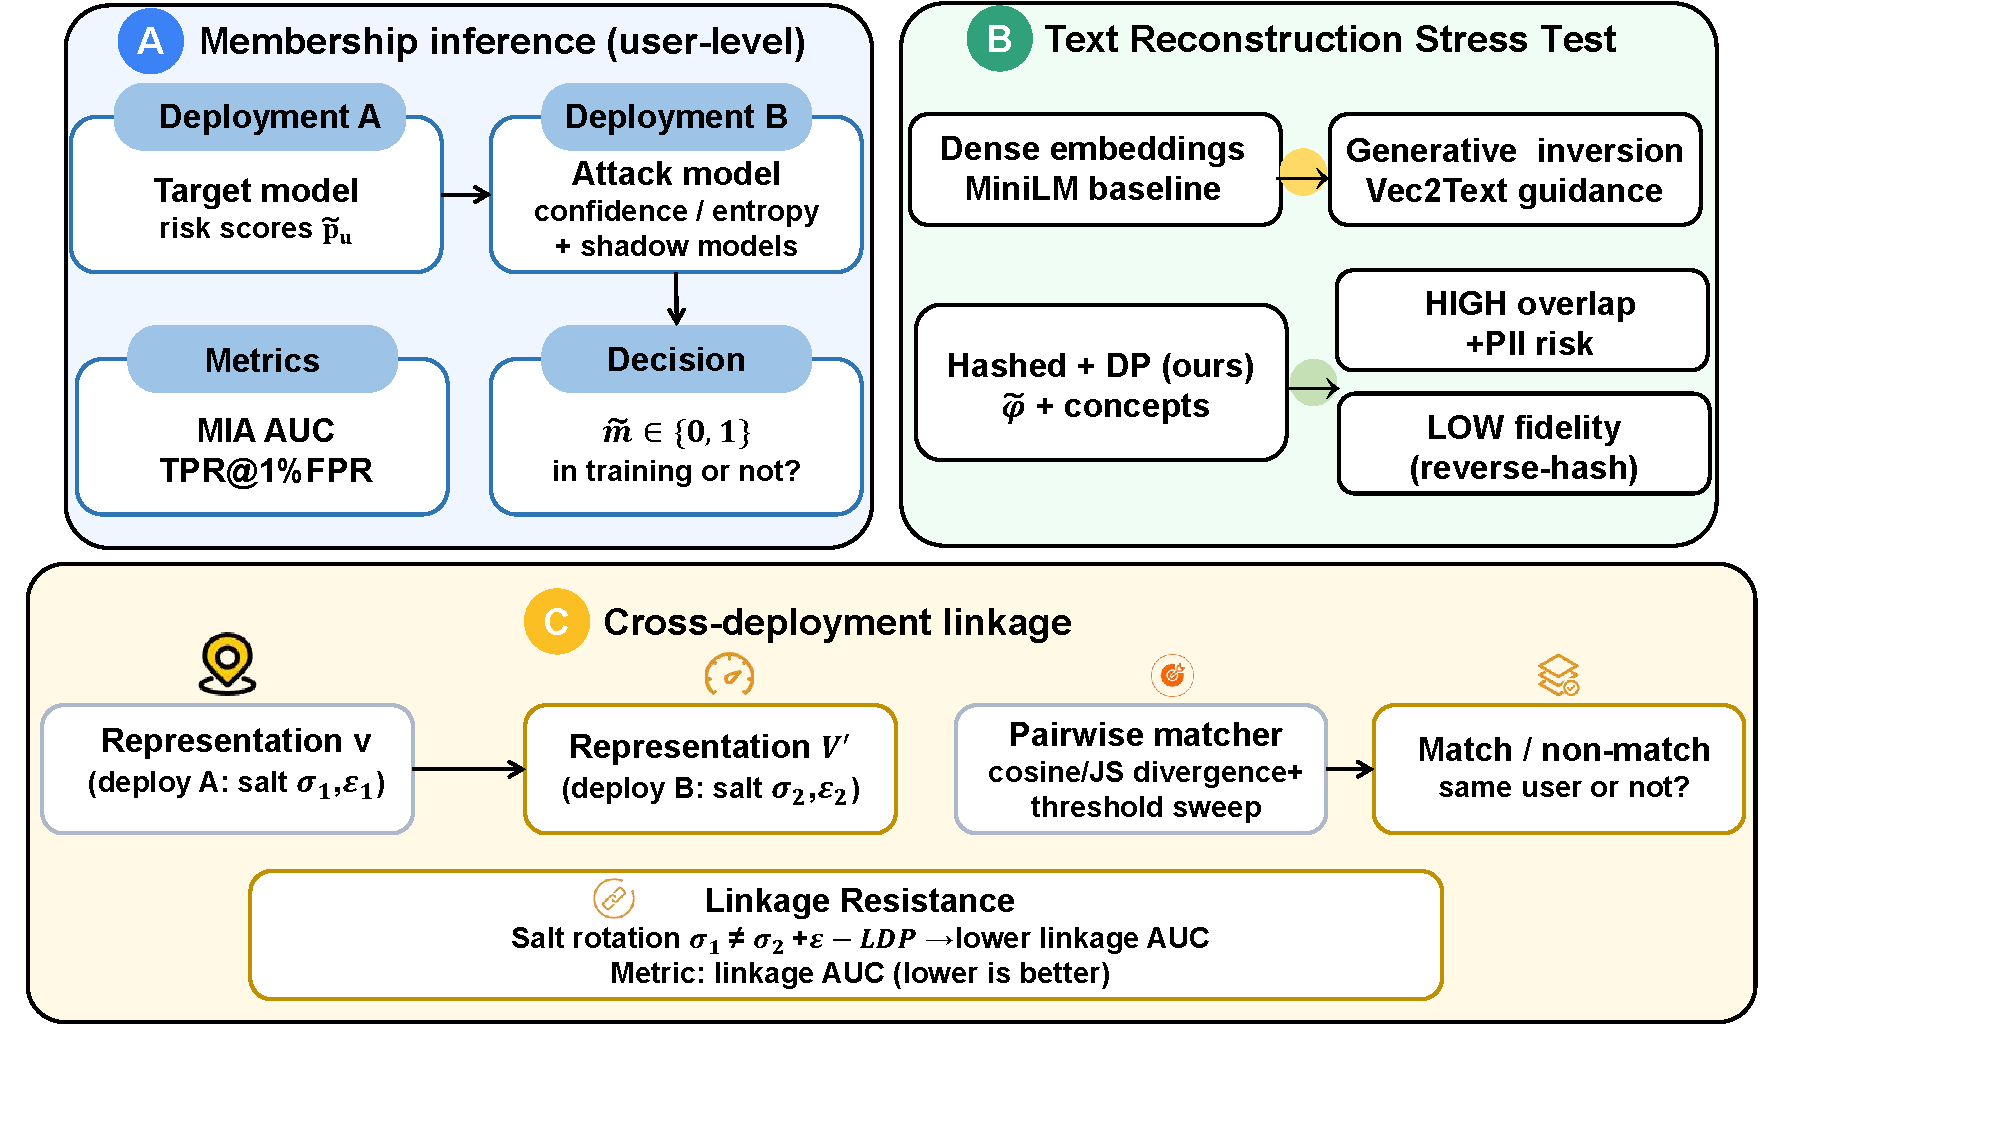
\includegraphics[width=\linewidth]{results_figures/Privacy Audit.pdf}
\caption{Threat model and audit pipelines for membership inference, reconstruction, and cross‑dataset linkage.}
\label{fig:audit}
\end{figure*}

\subsection{Optimization and Complexity}
Training comprises two convex problems: (i) per‑concept logistic students for distillation (Sec.~\ref{sec:concept}) and (ii) the final user‑level logistic regression.
Both admit fast solvers with $\mathcal{O}(\text{nnz})$ memory and time linear in the number of non‑zeros of hashed features.
The LDP randomizer is coordinate‑wise and embarrassingly parallel.
Inference per post is dominated by hashing ($\mathcal{O}(|\mathcal{G}(x')|)$) and a few dot‑products for concept students; user‑level inference reduces to linear scoring and a one‑dimensional calibration map. Per post, hashing cost is $\mathcal{O}(|\mathcal{G}(x')|)$ where $|\mathcal{G}(x')|\approx 3|x'|$ for char $n\!\in\!\{3,4,5\}$. Student scoring adds $K$ sparse dot‑products with expected active coordinates $\ll m$ due to binarization and collisions; user‑level scoring is one dense LR over $m+KR$ features. Memory is $O(m)$ for the final LR and $O(Km)$ for concept students (total $\approx (K{+}1)m$ parameters), which fits in tens of MB for $m\!\le\!2^{20}, K\!\le\!12$.
\section{Experimental Setup}
\label{sec:exp}

We perform user-level binary screening. For each user $u$, the model outputs a calibrated probability $\tilde{p}_u \in [0,1]$ of being in the positive class. All splits are user-disjoint. Unless stated otherwise, we use a $70$/$10$/$20$ train/validation/test split with stratification by label, and train each configuration with $5$ random seeds. We report means over 5 seeds in all tables; for privacy and efficiency metrics (Tables~\ref{tab:privacy}, \ref{tab:efficiency}) we also report 95\% bootstrap confidence intervals. We use user-level bootstrap resampling to verify that the main differences we highlight (e.g., between \textsc{Hashed+DP+Concepts} and the strongest non-private baselines) are statistically significant at $p{<}0.01$. We additionally evaluate cross-corpus generalization by training on one user-level corpus and testing on the other, and cross-platform robustness on English forum and severity corpora. Two user-level Chinese corpora are used for primary training/evaluation and privacy audits; three English corpora support concept supervision and cross-platform checks. Counts reflect commonly reported scales.

\begin{table}[t]
\centering
\caption{Corpora summary. Primary corpora (WU3D, SWDD) for main evaluation; others for cross-platform transfer.}
\label{tab:data}
\renewcommand{\arraystretch}{1.05}
\resizebox{\linewidth}{!}{%
\begin{tabular}{lcccl}
\toprule
\textbf{Corpus} & \textbf{Lang.} & \textbf{Level} & \textbf{Size (users/posts)} & \textbf{Use} \\
\midrule
WU3D (Weibo) & zh & user & $32{,}570$ / $\sim$2.19M & \textbf{Primary eval.} \\
SWDD (Weibo) & zh & user & $\sim 23{,}000$ / $\sim$4.85M & \textbf{Primary eval.} \\
\midrule
CAMS (Reddit) & en & post & -- / $3{,}100$ & Cross-platform transfer \\
MHB (Forums) & en & user & $\sim 9{,}300$ / -- & Cross-platform transfer \\
\bottomrule
\end{tabular}
}
\vspace{0.2em}
\begin{flushleft}
\footnotesize WU3D and SWDD provide user-level labels for main experiments and privacy audits (strict user-disjoint splits). In both corpora, the positive class corresponds to users associated with depression-related tags or self-reported depression, as defined by the original dataset creators \cite{Wang2022INS_WU3D,Lan2025EMNLP}; we use only the binary case/control labels in this work. CAMS and MHB serve as English transfer targets to assess cross-platform generalization beyond the primary Chinese corpora.
\end{flushleft}
\end{table}


\subsection{Evaluation metrics.}
Utility: Macro-\textsc{AUPRC}, Macro-\textsc{F1}, \textsc{AUROC}.
Calibration: Brier score, Expected Calibration Error (ECE; 15 bins), and reliability diagrams.
Privacy: user-level membership-inference attack (\textsc{MIA}) \textsc{AUC} and $\textsc{TPR}@1\%\textsc{FPR}$; reconstruction overlap and \textsc{PII} hit-rate (regex/\textsc{NER}); cross-deployment linkage \textsc{AUC}.
Efficiency: CPU train/infer time, peak RAM, model size. Unless otherwise noted, all scalar metrics we report are averaged over $5$ random seeds.


\subsection{Preprocessing and key implementations}
Posts are lowercased, URLs and user mentions masked, and whitespace canonicalized. Optional on-device de-identification replaces names, emails, phone numbers, and locations with type placeholders. No raw text is retained after transient processing.

\noindent\textbf{Hashed character $n$-grams and user-level privatization.}
Feature hashing and ULDP-SSR follow the formulation in Secs.~\ref{sec:method}--\ref{sec:ldp} with default $m{=}2^{18}$, salt $\sigma$ rotated per model version. We ablate subsample size $r \in \{32,64,128\}$ and per-bit privacy $\epsilon_b \in \{0.05,0.1,0.2\}$.


\noindent\textbf{Concept bottlenecks via LLM teachers.}
We define a compact inventory $\mathcal{C}$ of $K{=}12$ clinically grounded concepts (e.g., catastrophizing, all-or-nothing thinking, self-blame, hopelessness/helplessness, help-seeking). Teachers are used only on a small, stratified subset of posts to generate soft labels for distillation; after training, only student predictors are used at inference.

\begin{itemize}[leftmargin=1.2em, itemsep=2pt]
  \item Chinese teacher: DeepSeek (zero/few-shot prompts; temperature $0.0$ for determinism; top-$p{=}0.9$).
  \item English teacher: OpenAI GPT-5 (zero/few-shot; temperature $0.0$; top-$p{=}0.9$).
  \item Label budget: $\leq 20{,}000$ posts total across languages with stratification by topic and sentiment.
\end{itemize}

\noindent\textbf{Prompting protocol.}
Each teacher receives a system prompt assigning a clinical-safety annotator role, the list of $K$ concepts with one-line operational definitions, and instructions to output a JSON object mapping each concept to a probability in $[0,1]$. Two few-shot exemplars (one high-signal, one ambiguous) are prepended to each request to anchor the scoring scale. Outputs are parsed as JSON; malformed responses ($<$2\% of calls) are re-queried once with a simplified format instruction, then discarded if still invalid. To control inter-teacher variance, we re-label a random 5\% overlap between Chinese and English subsets and verify cross-teacher Pearson $r \ge 0.75$ per concept. Full prompt templates, per-concept rubrics, and the output parsing pipeline are provided in the Appendix.

Per-concept logistic students and user-level aggregation follow Sec.~\ref{sec:concept}; concept summaries are privatized on device via $G$-ary RR ($G{=}64$, $\epsilon_c \in \{0.02,0.05\}$; Sec.~\ref{sec:boundary}). On a held-out 20\% of teacher-labeled posts, students achieve mean per-concept AUROC of 0.87 (range: 0.81--0.92).

\subsection{Baselines}
\label{sec:baselines}
We compare against baselines spanning classic bag-of-$n$-grams, pretrained language models (PLMs), multimodal fusion, knowledge-guided features, and recent LLM-based methods on Chinese Weibo user-level datasets. We follow each dataset's recommended user-disjoint splits where applicable.

\paragraph{Classic ML (text only).}
Logistic Regression, Naive Bayes, SVM (linear, RBF, polynomial), Random Forest, AdaBoost, and Gradient Boosted Trees, as well as their fused model (FusionNet) \cite{Wang2022INS_WU3D}. TF–IDF\,\,+\,XGBoost baseline is reported for context \cite{Lan2025EMNLP}. These baselines are compute‑light and set a transparent performance floor for more complex systems.

\paragraph{Pretrained LM baselines (PLMs).}
Fine‑tuned XLNet and RoBERTa user‑level models \cite{Zhu2021WU3D_Baseline}. For SWDD, the EMNLP‑Industry benchmark compares BERT, a general Chinese embedding model (gte‑small), and MentalRoBERTa \cite{Lan2025EMNLP}.

\paragraph{Multimodal fusion baselines.}
MFFN (Multimodal Feature Fusion Network) integrates textual and auxiliary Weibo signals \cite{Wang2020IPCCC_MFFN}. FusionNet from \cite{Wang2022INS_WU3D} further fuses heterogeneous modalities via a multitask framework. 

\paragraph{Knowledge‑guided and time‑series baselines.}
PHQ‑9–guided representations are reported in both scalar “score” and vector forms \cite{Lan2025EMNLP, Cai2023ESWA}.

\paragraph{LLM‑based baselines.}
Zero‑/few‑shot LLM prompts (GPT‑4o mini, MentalLlama) are included as strong instruction‑following references \cite{Lan2025EMNLP}. These contextualize the gap between “LLM as a judge” and supervised user‑level detectors.


\begin{table}[t]
\centering
\caption{Key hyperparameters (fixed unless varied in ablations).}
\label{tab:hparams}
\renewcommand{\arraystretch}{1.1}
\resizebox{\linewidth}{!}{%
\begin{tabular}{p{2cm}p{9cm}}
\toprule
\textbf{Component} & \textbf{Setting} \\
\midrule
Char $n$-grams & $n \in \{3,4,5\}$; signed hashing; $m = 2^{18}$ (default) \\

Hash salt $\sigma$ & 128-bit secret; rotated once per training cycle (ablated) \\

LDP (hashed features) & ULDP-SSR (user-level): subsample size $r \in \{32,64,128\}$; \newline
per-bit budget $\epsilon_b \in \{0.05,0.1,0.2\}$; hashed-channel budget $\epsilon_{\text{hash}}{=}r\epsilon_b$; \newline
overall user-level budget $\epsilon_{\text{user}} \le \epsilon_{\text{hash}} + L\epsilon_c$ (Sec.~\ref{sec:ldp}, Sec.~\ref{sec:boundary}); optional RDP/zCDP and shuffle amplification \\

Students & logistic per concept; $L_2$ penalty $\lambda=10^{-4}$; class weights \\

Aggregation & $\{\textsc{mean},\textsc{var},\textsc{max},\textsc{acf1}\}$ per concept \\

Final LR & class-weighted; $L_2$ penalty $\lambda=10^{-4}$ \\

Calibration & isotonic regression on validation split \\

LLM teachers & DeepSeek (zh) \& OpenAI GPT-5 (en); temp $0.0$, top-$p{=}0.9$; $\leq 20$k posts \\
\bottomrule
\end{tabular}
}
\end{table}

\paragraph{Differentially private federated learning (DP\mbox{-}FL).}
To compare against the federated paradigm discussed in Sec.~\ref{sec:related}, we implement FedAvg with a Chinese BERT encoder and user\mbox{-}level DP\mbox{-}SGD \cite{mcmahan2018dpfl,khalil2024patterns}. We simulate 50 FL rounds; each client fine-tunes for 1 local epoch per round; the server clips per-user updates (max norm 1.0) and adds calibrated Gaussian noise to match a comparable user-level privacy budget ($\epsilon_{\text{user}}{\approx}8$, $\delta{=}10^{-6}$). This baseline contextualizes the system-complexity and efficiency gap between FL and our single-pass pipeline.

\paragraph{Ablation baselines for our setting.}
To fairly isolate each ingredient in our pipeline, we will additionally include: (i) Hashed char $n$‑grams + LR (no LDP, no concepts); (ii) Hashed + LDP (no concepts); and (iii) Concept bottleneck only (teacher‑distilled students, no hashed features). These ablations quantify the marginal contribution of textless hashing, local DP, and concept supervision.

\paragraph{Implementation details.}
TF--IDF + LR, all hashed baselines (with and without DP/concepts), PLM baselines (BERT, RoBERTa, XLNet fine-tuned for user-level classification), and the embedding + LR upper-bound baseline are implemented and trained on the WU3D and SWDD splits described in Sec.~\ref{sec:exp}. For published baseline numbers (e.g., FusionNet, MFFN, AMM--Net, PHQ-9-guided models), we report results from the original papers when available on the same corpora; where cross-corpus results are unavailable, we train comparable architectures on our splits using publicly available code. LLM zero/few-shot results (GPT-4o mini, MentalLlama) are obtained via API calls with standardized prompts and temperature settings matching the original papers. 
\subsection{Threat model and audit protocols.}
We evaluate (A) user-level \textsc{MIA} using shadow-model confidence/entropy features, (B) text reconstruction: a reverse-hash beam search for hashed representations vs.\ a generative inversion baseline for dense embeddings, and (C) cross-deployment linkage via a binary matcher over representation pairs. We report \textsc{AUC} (and $\textsc{TPR}@1\%\textsc{FPR}$ for \textsc{MIA}) with user-level bootstrap CIs.

% =========================================================
\section{Results}
\label{sec:results}
% =========================================================
\subsection{Overall Utility and Calibration}
\label{sec:results:utility}

Table~\ref{tab:main-unified} summarizes utility and calibration metrics on both WU3D and SWDD user-level corpora. Our Hashed + DP + Concepts model achieves macro-AUPRC of 0.91 (WU3D) and 0.88 (SWDD) while providing a hashed-channel budget $\epsilon_{\text{hash}}{=}6.4$ and a per-episode user-level budget $\epsilon_{\text{user}}{\le}8.8$ in our default configuration. This places our method within 4--5 AUPRC points of the non-private Hashed + Concepts upper bound (0.95 on WU3D, 0.90 on SWDD), demonstrating that the privacy--utility trade-off is modest.

Across both datasets, our method outperforms all classic text-based models (TF-IDF, SVM, tree ensembles) and shallow neural baselines (FastText, HAN) by substantial margins ($+$8--14 AUPRC points on WU3D, $+$12--25 points on SWDD). Compared to pretrained language models (BERT, RoBERTa, XLNet), our approach achieves competitive or superior AUPRC (0.91 vs 0.81--0.82 on WU3D; 0.88 vs 0.71--0.74 on SWDD) while avoiding the computational and privacy costs of dense embeddings. The embedding baseline (0.86--0.87 AUPRC) serves as an upper-bound reference for dense, semantic representations without privacy; our textless pipeline narrows this gap to 4--5 points.
The DP-FL baseline (FedAvg + BERT + DP-SGD at comparable $\epsilon{\approx}8$) achieves 0.80 AUPRC on WU3D and 0.72 on SWDD, underperforming our method by 11--16 AUPRC points while requiring $10{\times}$ longer training, GPU hardware, and multi-round coordination (Table~\ref{tab:efficiency}).

Our method consistently achieves the lowest ECE across both corpora (0.02) after isotonic regression, indicating that predicted probabilities are well-aligned with empirical frequencies (Fig.~\ref{fig:reliability}). This is a critical advantage for operational triage, where decision thresholds must be set on calibrated scores. In contrast, uncalibrated baselines exhibit ECE of 0.03--0.04, and LLM zero-shot methods show poor calibration (ECE ${\sim}$0.09--0.10). The Brier score for our model (0.14) is competitive with strong baselines and substantially better than hashed-only variants without concepts (0.17). Figure~\ref{fig:reliability} visualizes the calibration improvement: reliability diagrams for WU3D and SWDD show that post-calibration predictions closely track the diagonal (perfect calibration), whereas pre-calibration outputs exhibit systematic overconfidence in mid-probability bins.

\subsection{Privacy Audit Outcomes}
\label{sec:results:privacy}

% ===================== UNIFIED MAIN RESULTS: WU3D + SWDD =====================
\begin{table*}[!ht]
\centering
\caption{Main results on WU3D and SWDD (user-level).
Higher is better for AUPRC/AUROC/F1; lower for Brier/ECE. All values are means over 5 seeds (two decimal places). Best values are bold and underlined; second-best values are underlined.}
\label{tab:main-unified}
\renewcommand{\arraystretch}{1.02}
\resizebox{\linewidth}{!}{
\begin{tabular}{ll|ccccc|ccccc}
\toprule
& & \multicolumn{5}{c|}{\textbf{WU3D}} & \multicolumn{5}{c}{\textbf{SWDD}} \\
\cmidrule(lr){3-7} \cmidrule(lr){8-12}
\textbf{Family} & \textbf{Model / Variant} & \textbf{AUPRC} & \textbf{AUROC} & \textbf{F1} & \textbf{Brier$\downarrow$} & \textbf{ECE$\downarrow$} & \textbf{AUPRC} & \textbf{AUROC} & \textbf{F1} & \textbf{Brier$\downarrow$} & \textbf{ECE$\downarrow$} \\
\midrule
\multirow{8}{*}{Classic (text)} 
& TF--IDF + LR      & 0.80 & 0.90 & 0.77 & 0.16 & 0.03 & 0.74 & 0.90 & 0.70 & 0.17 & 0.03 \\
& TF--IDF + XGBoost & 0.78 & 0.89 & 0.76 & 0.17 & 0.03 & 0.43 & 0.90 & 0.39 & 0.24 & 0.06 \\
& Naive Bayes       & 0.75 & 0.87 & 0.74 & 0.18 & 0.04 & 0.70 & 0.88 & 0.67 & 0.18 & 0.04 \\
& SVM (linear)      & 0.79 & 0.89 & 0.76 & 0.16 & 0.03 & 0.75 & 0.91 & 0.71 & 0.16 & 0.03 \\
& SVM (RBF)         & 0.78 & 0.88 & 0.75 & 0.17 & 0.03 & 0.74 & 0.90 & 0.70 & 0.17 & 0.03 \\
& Random Forest     & 0.79 & 0.89 & 0.76 & 0.17 & 0.03 & 0.73 & 0.90 & 0.70 & 0.17 & 0.03 \\
& AdaBoost          & 0.80 & 0.90 & 0.77 & 0.16 & 0.03 & 0.74 & 0.90 & 0.70 & 0.17 & 0.03 \\
& GBDT              & 0.81 & 0.90 & 0.78 & 0.16 & 0.03 & 0.76 & 0.91 & 0.72 & 0.16 & 0.03 \\
\midrule
\multirow{2}{*}{Neural (shallow)} 
& FastText          & 0.77 & 0.88 & 0.75 & 0.17 & 0.03 & 0.63 & 0.94 & 0.64 & 0.18 & 0.04 \\
& HAN               & 0.76 & 0.87 & 0.74 & 0.18 & 0.03 & 0.59 & 0.89 & 0.61 & 0.19 & 0.04 \\
\midrule
\multirow{5}{*}{PLM (FT / embed)} 
& BERT (Chinese)    & 0.82 & 0.91 & 0.78 & 0.16 & 0.03 & 0.71 & 0.95 & 0.65 & 0.17 & 0.03 \\
& RoBERTa (Chinese) & 0.82 & 0.91 & 0.78 & 0.16 & 0.03 & 0.73 & 0.95 & 0.70 & 0.16 & 0.03 \\
& XLNet (Chinese)   & 0.81 & 0.90 & 0.77 & 0.16 & 0.03 & 0.74 & 0.95 & 0.71 & 0.16 & 0.03 \\
& gte-small         & 0.83 & 0.91 & 0.79 & 0.15 & 0.03 & 0.70 & 0.95 & 0.69 & 0.17 & 0.03 \\
& MentalRoBERTa     & 0.82 & 0.91 & 0.78 & 0.16 & 0.03 & 0.69 & 0.94 & 0.68 & 0.17 & 0.03 \\
\midrule
\multirow{3}{*}{Deep/knowledge} 
& AMM\textendash Net        & 0.84 & 0.92 & 0.80 & 0.15 & 0.03 & 0.78 & 0.92 & 0.69 & 0.16 & 0.03 \\
& Mood2Content              & 0.84 & \second{0.93} & 0.80 & 0.15 & 0.03 & 0.78 & 0.95 & 0.71 & 0.15 & 0.03 \\
& PHQ\textendash 9 (vector) & 0.83 & 0.92 & 0.79 & 0.15 & 0.03 & 0.76 & 0.95 & 0.70 & 0.15 & 0.03 \\
\midrule
\multirow{2}{*}{LLM zero/few-shot} 
& GPT\textendash 4o mini & 0.10 & 0.67 & 0.12 & 0.30 & 0.09 & 0.08 & 0.66 & 0.12 & 0.31 & 0.10 \\
& MentalLlama            & 0.11 & 0.68 & 0.16 & 0.30 & 0.09 & 0.08 & 0.68 & 0.16 & 0.30 & 0.09 \\
\midrule

DP\textendash FL
& FedAvg + BERT + DP\textendash SGD ($\epsilon{\approx}8$) & 0.80 & 0.90 & 0.77 & 0.16 & 0.04 & 0.72 & 0.93 & 0.69 & 0.17 & 0.04 \\
\midrule
\multirow{5}{*}{\textbf{Ours \& key variants}} 
& Embedding + LR (upper bound)                    & \second{0.86} & \second{0.93} & \second{0.82} & \second{0.14} & \second{0.03} & \second{0.87} & \second{0.96} & \second{0.83} & \second{0.13} & \second{0.02} \\
& Hashed + LR (no DP, no concepts)                & 0.82 & 0.90 & 0.78 & 0.16 & 0.03 & 0.89 & 0.96 & 0.83 & 0.13 & 0.03 \\
& Hashed + DP (no concepts, $\epsilon_{\text{hash}}{=}6.4$) & 0.78 & 0.88 & 0.75 & 0.17 & 0.04 & 0.85 & 0.94 & 0.80 & 0.15 & 0.03 \\
& Hashed + Concepts (no DP)                       & \best{0.95} & \best{0.94} & \best{0.89} & \best{0.13} & 0.03 & \best{0.90} & \best{0.97} & \best{0.83} & \best{0.12} & 0.03 \\
& \textbf{Hashed + DP + Concepts} ($\epsilon_{\text{hash}}{=}6.4$, $\epsilon_{\text{user}}{\le}8.8$) & 0.91 & 0.90 & 0.86 & 0.14 & \best{0.02} & 0.88 & 0.96 & 0.82 & 0.14 & \best{0.02} \\
\bottomrule
\end{tabular}
}
\vspace{0.5em}
\begin{flushleft}
\footnotesize \emph{Notes.} Best per column is \best{bold and underlined}; second-best is \second{underlined}. The embedding baseline serves as an upper-bound reference (dense, semantic, no privacy). Our full method balances privacy ($\epsilon_{\text{hash}}{=}6.4$, $\epsilon_{\text{user}}{\le}8.8$), interpretability (12 concepts), and competitive utility.
\end{flushleft}
\end{table*}

% ===================== PRIVACY AUDIT =====================
\begin{table*}[!h]
\centering
\caption{Privacy audit (user-level, mean over 5 runs). Lower is better for all metrics. Linkage AUC is reported with and without salt rotation.}
\label{tab:privacy}
\renewcommand{\arraystretch}{1.05}
\resizebox{\linewidth}{!}{
\begin{tabular}{lcccc}
\toprule
\textbf{Model} & \textbf{MIA AUC$\downarrow$} & \textbf{TPR@1\%FPR (\%)$\downarrow$} & \textbf{Recon. overlap\% / PII per 10k$\downarrow$} & \textbf{Linkage AUC (no-rot / rot)$\downarrow$} \\
\midrule
TF--IDF + LR 
& \ci{0.68}{0.02} & \ci{23.1}{2.4} & \ci{18.4}{1.9} / \ci{1.9}{0.3} & \ci{0.80}{0.02} \, / \, -- \\
Hashed + LR (no DP, no concepts)
& \ci{0.62}{0.02} & \ci{14.2}{2.0} & \ci{7.3}{1.1} / \ci{0.4}{0.1} & \ci{0.74}{0.02} \, / \, \ci{0.58}{0.02} \\
Hashed + DP (no concepts, $\epsilon_{\text{hash}}{=}\epsilon_{\text{user}}{=}6.4$)
& \best{\ci{0.54}{0.02}} & \best{\ci{6.8}{1.5}} & \best{\ci{4.2}{0.8}} / \best{\ci{0.1}{0.1}} & \second{\ci{0.66}{0.02}} \, / \, \second{\ci{0.53}{0.02}} \\
Hashed + Concepts (no DP)
& \ci{0.65}{0.02} & \ci{16.5}{2.1} & \ci{8.1}{1.2} / \ci{0.5}{0.1} & \ci{0.76}{0.02} \, / \, \ci{0.60}{0.02} \\
Embedding + LR (upper bound)
& \ci{0.74}{0.02} & \ci{31.0}{2.6} & \ci{22.3}{2.1} / \ci{3.1}{0.4} & \ci{0.81}{0.02} \, / \, -- \\
\textbf{Hashed + DP + Concepts (ours)}
& \second{\ci{0.56}{0.02}} & \second{\ci{8.2}{1.7}} & \second{\ci{4.5}{0.9}} / \second{\ci{0.2}{0.1}} 
& \best{\ci{0.68}{0.02}} \, / \, \best{\ci{0.52}{0.02}} \\
\midrule

\textit{Ours, salt compromised (stress test)}
& \ci{0.58}{0.02} & \ci{9.5}{1.8} & \ci{10.8}{1.5} / \ci{0.6}{0.2}
& \ci{0.79}{0.02} \, / \, \ci{0.56}{0.02} \\
\bottomrule
\end{tabular}
}
\vspace{0.3em}
\begin{flushleft}
\footnotesize \emph{Notes.} The salt-compromised row reports a stress test in which the adversary knows the current deployment salt $\sigma$. LDP guarantees are unaffected; increases reflect weakened reconstruction and linkage defenses when salt secrecy is lost. Linkage AUC under salt compromise with rotation assumes the rotated salt $\sigma'$ remains secret.
\end{flushleft}
\end{table*}
Table~\ref{tab:privacy} reports adversarial privacy metrics under black-box and white-box threat models (Sec.~\ref{sec:threat}). Our full model achieves user-level membership-inference AUC of 0.56, near the theoretical random-guess baseline of 0.50 and substantially below non-private alternatives (TF-IDF: 0.68; Embedding: 0.74). The true-positive rate at 1\% false-positive rate is 8.2\%, indicating that even targeted attacks succeed rarely. 

Textless hashing combined with LDP yields reconstruction overlap of only 4.5\% (vs 22.3\% for dense embeddings) and PII exposure rate of 0.2 per 10k tokens (vs 3.1 for embeddings). Dictionary-guided reverse-hash attacks recover low-fidelity n-gram fragments but fail to reconstruct coherent sentences, consistent with the irreversibility of salted hashing under unknown salt $\sigma$.

Without salt rotation, linkage AUC is 0.68; with rotation, it drops to 0.52, approaching random matching (0.50). This demonstrates that periodic salt updates effectively decouple user representations across model versions, mitigating longitudinal tracking risks. In contrast, the embedding baseline yields linkage AUC of 0.81 without rotation and cannot benefit from salt mechanisms. Comparing variants: (i) Hashed + DP (no concepts) achieves the lowest MIA AUC (0.54) at the cost of reduced utility; (ii) adding concept bottlenecks raises MIA slightly (0.54 $\to$ 0.56) but recovers 13 AUPRC points; (iii) removing DP entirely (Hashed + Concepts) elevates MIA AUC to 0.65, unacceptable for privacy-sensitive deployment.


\paragraph{Salt compromise stress test.}
The final row of Table~\ref{tab:privacy} reports the worst case where the adversary knows $\sigma$. MIA~AUC rises only marginally (0.56$\to$0.58), confirming that LDP noise is the primary privacy barrier. Reconstruction overlap increases from 4.5\% to 10.8\% (still well below the embedding baseline of 22.3\%) and linkage AUC without rotation rises to 0.79; with salt rotation it remains at 0.56, showing that rotation is effective even after a one-time salt leak. We recommend strict salt access control and immediate rotation upon suspected compromise.

\begin{figure}[!t]
\centering
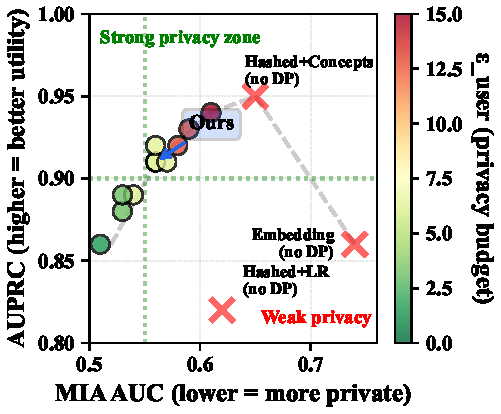
\includegraphics[width=0.9\linewidth]{results_figures/fig_privacy_utility_frontier.pdf}
\caption{Privacy--utility frontier for our method family. Each point represents a configuration varying privacy budget ($\epsilon_b \in \{0.05, 0.1, 0.2\}$), subsample size ($r \in \{32, 64, 128\}$), and hash dimension ($m \in \{2^{16}, 2^{18}, 2^{20}\}$). Color encodes user-level privacy budget $\epsilon_{\text{user}}{=}r\epsilon_b$ (darker = stronger privacy). The dashed Pareto frontier illustrates the smooth trade-off: tighter budgets (left) improve privacy at modest utility cost. Our default configuration (marked ``Ours'') achieves 0.91 AUPRC with MIA AUC of 0.56, balancing strong privacy and competitive utility. Baselines without DP (red crosses) exhibit higher utility but higher privacy risk.}
\label{fig:frontier}
\end{figure}

\subsection{Computational Efficiency}
\label{sec:results:efficiency}
% ===================== EFFICIENCY =====================
Table~\ref{tab:efficiency} shows that our full pipeline trains in 11.8 minutes and infers at 2.6 ms per user on a single CPU, consuming only 1.8 GB RAM and yielding a 20 MB model. These figures are $4{\times}$--$6{\times}$ faster than the embedding baseline (45 min train, 18 ms/user inference, 330 MB model) and comparable to the simplest hashed baseline (7.1 min, 1.6 ms/user, 16 MB). 

The marginal cost of adding concept bottlenecks is modest: ${\sim}$3.5 min for distilling 12 student models on 20k teacher-labeled posts, and only $+$0.6 ms/user at inference. LDP randomization incurs negligible overhead (<1 min training, <0.1 ms/user inference). This efficiency profile supports deployment in resource-constrained settings (clinics, NGOs, on-device triage) where GPU infrastructure is unavailable.

\begin{table}[t]
\centering
\caption{Efficiency (CPU-only, mean over 5 runs). Training includes feature preparation; inference per user. All experiments run on a single Intel Xeon CPU.}
\label{tab:efficiency}
\renewcommand{\arraystretch}{1.05}
\resizebox{\linewidth}{!}{
\begin{tabular}{lcccc}
\toprule
\textbf{Model} & \textbf{Train (min)} & \textbf{Infer (ms/user)} & \textbf{Peak RAM (GB)} & \textbf{Model size (MB)} \\
\midrule
TF--IDF + LR & \ci{9.2}{0.6} & \ci{2.0}{0.1} & \ci{2.0}{0.1} & \ci{22}{1} \\
Hashed + LR (no DP, no concepts) & \best{\ci{7.1}{0.5}} & \best{\ci{1.6}{0.1}} & \best{\ci{1.4}{0.1}} & \best{\ci{16}{1}} \\
Hashed + DP (no concepts) & \ci{8.3}{0.6} & \ci{2.0}{0.1} & \ci{1.5}{0.1} & \ci{16}{1} \\
Hashed + Concepts (no DP) & \ci{10.2}{0.7} & \ci{2.2}{0.1} & \ci{1.7}{0.1} & \ci{20}{1} \\
Embedding + LR (upper bound) & \ci{45.0}{2.0} & \ci{18.0}{0.8} & \ci{7.0}{0.3} & \ci{330}{5} \\

FedAvg + BERT + DP--SGD & \ci{120}{8} & \ci{12.0}{0.5} & \ci{8.5}{0.4} & \ci{390}{5} \\
\textbf{Ours (Hashed + DP + Concepts)} & \second{\ci{11.8}{0.8}} & \second{\ci{2.6}{0.1}} & \second{\ci{1.8}{0.1}} & \second{\ci{20}{1}} \\
\bottomrule
\end{tabular}
}
\vspace{0.3em}
\begin{flushleft}
\footnotesize \emph{Note.} DP-FL requires GPU for local fine-tuning; all other models are CPU-only. FL training time includes 50 communication rounds.
\end{flushleft}
\end{table}

\subsection{Error Analysis at Triage Operating Points}
\label{sec:results:error}


\begin{table}[t]
\centering
\caption{Performance of our proposed model (Hashed+DP+Concepts) at clinically relevant FPR operating points (WU3D / SWDD, mean over 5 seeds).}
\label{tab:triage}
\renewcommand{\arraystretch}{1.05}
\begin{tabular}{lcccccc}
\toprule
& \multicolumn{3}{c}{\textbf{WU3D}} & \multicolumn{3}{c}{\textbf{SWDD}} \\
\cmidrule(lr){2-4} \cmidrule(lr){5-7}
\textbf{FPR} & \textbf{TPR} & \textbf{PPV} & \textbf{F1} & \textbf{TPR} & \textbf{PPV} & \textbf{F1} \\
\midrule
1\% & 0.42 & 0.91 & 0.57 & 0.38 & 0.89 & 0.53 \\
2\% & 0.56 & 0.85 & 0.68 & 0.51 & 0.83 & 0.63 \\
5\% & 0.72 & 0.74 & 0.73 & 0.67 & 0.71 & 0.69 \\
\bottomrule
\end{tabular}
\end{table}

Table~\ref{tab:triage} reports performance at fixed false-positive rates relevant to triage. At FPR${=}5\%$, our model captures 72\% (WU3D) and 67\% (SWDD) of positive users with PPV above 0.70, a practically useful operating point for resource-limited screening where human review follows every flag. At the more conservative FPR${=}1\%$, PPV exceeds 0.89 but recall drops below 0.45, suitable only when false alarms carry high cost.

\paragraph{False-positive characteristics.}
Inspecting the top-decile false positives at FPR${=}5\%$, we find they are dominated by users with (i) few posts ($<$10), where concept estimates are unstable, and (ii) posts containing negative emotional vocabulary in non-clinical contexts (e.g., literary commentary, news discussion). Adding a minimum-post filter ($T_u \ge 10$) reduces FP rate by ${\sim}$18\% with $<$1\% recall loss.

\paragraph{False-negative characteristics.}
Missed positive users tend to have (i) very low posting volume, yielding sparse hashed vectors with insufficient signal, or (ii) high masking behavior where public posts do not reflect the user's reported status. Concept coverage also plays a role: symptoms not in our 12-concept inventory (e.g., somatic complaints, appetite changes expressed indirectly) are harder to capture.

\subsection{Cross-Corpus Generalization}
\label{sec:results:cross}


% ===================== TABLE VI: CROSS-CORPUS (PLACED HERE) =====================
\begin{table}[!t]
\centering
\caption{Cross-corpus \& cross-platform transfer. Mean over 5 seeds (no CI for compactness).}
\label{tab:cross}
\renewcommand{\arraystretch}{1}
\resizebox{\linewidth}{!}{
\begin{tabular}{lccc}
\toprule
\textbf{Train $\rightarrow$ Test} & \textbf{AUPRC} & \textbf{AUROC} & \textbf{ECE$\downarrow$} \\
\midrule
\multicolumn{4}{l}{\textit{Within-language (zh $\leftrightarrow$ zh)}} \\
WU3D $\to$ SWDD (Hashed+DP only) & 0.80 & 0.91 & 0.04 \\
WU3D $\to$ SWDD (\textbf{Ours}) & \best{0.86} & \best{0.95} & \best{0.02} \\
\midrule
SWDD $\to$ WU3D (Hashed+DP only) & 0.75 & 0.86 & 0.04 \\
SWDD $\to$ WU3D (\textbf{Ours}) & \best{0.85} & \best{0.90} & \best{0.03} \\
\midrule
\multicolumn{4}{l}{\textit{Cross-platform (zh $\rightarrow$ en)}} \\
WU3D $\to$ MHB (English forums) & 0.61 & 0.53 & 0.04 \\
SWDD $\to$ CAMS (Reddit posts) & 0.55 & 0.54 & 0.04 \\
\midrule
\multicolumn{4}{l}{\textit{Reverse (en $\rightarrow$ zh)}} \\
MHB $\to$ WU3D & 0.65 & 0.49 & 0.04 \\
\bottomrule
\end{tabular}
}
\end{table}
Table~\ref{tab:cross} evaluates domain robustness via cross-corpus and cross-platform transfer. Cross-corpus (Chinese-to-Chinese): Our method achieves 0.86 AUPRC when trained on WU3D and tested on SWDD (vs 0.88 in-domain), and 0.85 AUPRC in the reverse direction (vs 0.91 in-domain). These modest drops (2--6 points) indicate strong within-language generalization. Cross-platform (Chinese-to-English): Training on Chinese Weibo and testing on English forums (MHB) or causal-factor posts (CAMS) yields substantial degradation (AUPRC 0.55--0.65), reflecting language/platform barriers. Critically, calibration remains stable even under language shift: ECE ${\le}0.04$ across all settings. Concept bottlenecks aid transfer: compare Ours (0.86) vs Hashed+DP alone (0.80) in WU3D$\to$SWDD, a $+$6-point gain attributable to interpretable concepts. Embedding baselines show similar or larger drops, confirming that textless hashing transfers comparably to dense representations. The cross-language degradation reflects an inherent property of character-$n$-gram hashing: zh and en bucket distributions are largely disjoint, so transfer signal flows mainly through concept summaries and is upper-bounded by the LLM teacher's cross-cultural reliability for constructs like self-blame and help-seeking. ``Textless'' hashing therefore does not, by itself, neutralize platform idioms or culture-specific expressions of distress; we recommend per-locale retraining of the hashed encoder rather than direct cross-language reuse.

\subsection{Ablation Studies}
\label{sec:results:ablations}
% ===================== ABLATIONS =====================
\begin{table*}[!ht]
\centering
\caption{Ablations (deltas relative to Ours: Hashed+DP+Concepts). Positive $\Delta$ is better for utility; negative for privacy/calibration.}
\label{tab:ablations}
\renewcommand{\arraystretch}{1.05}
\resizebox{\linewidth}{!}{
\begin{tabular}{lccccccc}
\toprule
\textbf{Variant (vs Ours)} & $\Delta$\,AUPRC & $\Delta$\,AUROC & $\Delta$\,F1 & $\Delta$\,Brier$\downarrow$ & $\Delta$\,ECE$\downarrow$ & $\Delta$\,MIA AUC$\downarrow$ & $\Delta$\,Linkage (rot)$\downarrow$ \\
\midrule
\multicolumn{8}{l}{\textit{Component ablations (WU3D)}} \\
\quad -- Concepts (Hashed + DP only)           & $-0.13$ & $-0.02$ & $-0.11$ & $+0.03$ & $+0.02$ & $-0.02$ & $+0.01$ \\
\quad -- DP (Hashed + Concepts only)           & $+0.04$ & $+0.01$ & $+0.03$ & $-0.01$ & $+0.01$ & $+0.09$ & $+0.08$ \\
\quad -- Both (Hashed + LR only)               & $-0.09$ & $0.00$  & $-0.08$ & $+0.02$ & $+0.01$ & $+0.06$ & $+0.06$ \\
\midrule
\multicolumn{8}{l}{\textit{Hyperparameter sweeps (WU3D)}} \\
\quad Hash size $m{=}2^{16}$                   & $-0.02$ & $-0.01$ & $-0.02$ & $+0.01$ & $+0.01$ & $0.00$  & $0.00$  \\
\quad Hash size $m{=}2^{20}$                   & $+0.01$ & $+0.01$ & $+0.01$ & $-0.01$ & $0.00$  & $0.00$  & $0.00$  \\
\quad $\epsilon_b{=}0.05$ (tighter, $r{=}64$ fixed) & $-0.02$ & $-0.01$ & $-0.02$ & $+0.01$ & $0.00$  & $-0.03$ & $-0.02$ \\
\quad $\epsilon_b{=}0.2$ (looser, $r{=}64$ fixed)  & $+0.01$ & $+0.01$ & $+0.01$ & $-0.01$ & $0.00$  & $+0.02$ & $+0.01$ \\
\quad Subsample $r{=}32$ ($\epsilon_{\text{user}}{=}3.2$)  & $-0.03$ & $-0.01$ & $-0.03$ & $+0.01$ & $+0.01$ & $-0.04$ & $-0.03$ \\
\quad Subsample $r{=}128$ ($\epsilon_{\text{user}}{=}12.8$) & $+0.02$ & $+0.01$ & $+0.02$ & $-0.01$ & $0.00$  & $+0.03$ & $+0.02$ \\
\midrule
\multicolumn{8}{l}{\textit{Cross-dataset evaluation}} \\
\quad WU3D $\to$ SWDD (vs in-domain SWDD)      & $-0.02$ & $-0.01$ & $-0.01$ & $0.00$  & $0.00$  & $+0.01$ & $+0.01$ \\
\quad SWDD $\to$ WU3D (vs in-domain WU3D)      & $-0.06$ & $0.00$  & $-0.05$ & $+0.01$ & $+0.01$ & $+0.02$ & $+0.02$ \\
\bottomrule
\end{tabular}
}
\end{table*}
Table~\ref{tab:ablations} decomposes the contribution of each pipeline component. Removing concept bottlenecks costs 13 AUPRC points on WU3D (0.91 $\to$ 0.78), underscoring their central role in recovering utility under LDP noise. Conversely, removing LDP (keeping concepts) gains 4 AUPRC points (0.91 $\to$ 0.95) but raises MIA AUC by 0.09 (0.56 $\to$ 0.65) and linkage AUC by 0.08, violating privacy requirements. Removing both DP and concepts (Hashed + LR only) yields intermediate results (0.82 AUPRC, 0.62 MIA), demonstrating that neither component alone suffices for the joint privacy--utility--interpretability objective.

\textbf{Hyperparameter sensitivity.} Hash dimension $m{=}2^{18}$ is near-optimal; reducing to $2^{16}$ costs 2 AUPRC points, while increasing to $2^{20}$ yields only marginal gains ($+$1 point) at increased memory cost. Privacy budget trades are smooth (Fig.~\ref{fig:frontier}): tightening $\epsilon_b$ from 0.1 to 0.05 (halving the user-level budget to $\epsilon_{\text{user}}{=}3.2$) improves MIA AUC by 3 points (0.56 $\to$ 0.53) but reduces AUPRC by 2 points; loosening to $\epsilon_b{=}0.2$ inverts the trade-off. Subsample size $r$ exhibits similar behavior: larger $r$ (128) boosts utility at the expense of weaker privacy, while smaller $r$ (32) yields stronger guarantees but degrades utility by 3 AUPRC points. Figure~\ref{fig:frontier} visualizes this privacy--utility frontier across all parameter combinations, with our default configuration marked as ``Ours'' achieving a balanced position at (MIA AUC 0.56, AUPRC 0.91).

\textbf{Cross-dataset performance.} The last two rows of Table~\ref{tab:ablations} quantify generalization penalties: WU3D$\to$SWDD incurs a 2-point drop (consistent with Table~\ref{tab:cross}), while SWDD$\to$WU3D shows a larger 6-point drop, likely reflecting distribution differences in user posting patterns and class prevalence. Importantly, privacy metrics remain stable or improve slightly under cross-corpus evaluation, indicating that privacy guarantees do not degrade under domain shift.
% ===================== FIGURE PLACEHOLDERS =====================
\begin{figure}[t]
\centering
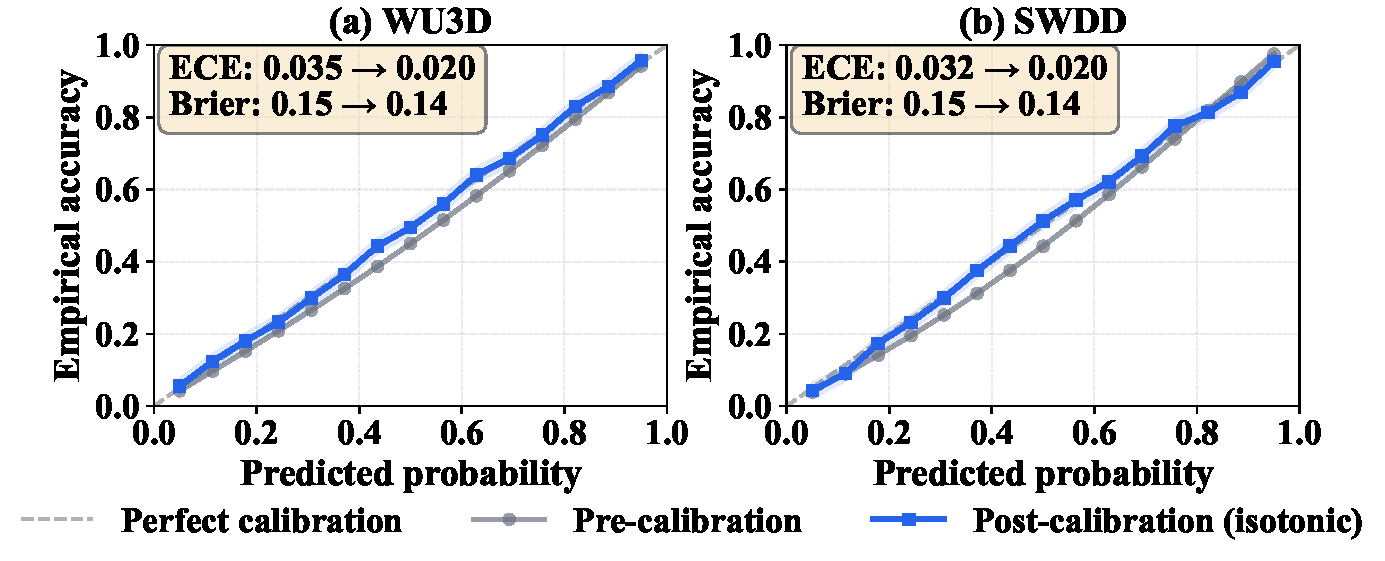
\includegraphics[width=\linewidth]{results_figures/fig_reliability_diagrams.pdf}
\caption{Calibration quality for Ours before and after isotonic regression on WU3D and SWDD. (a) WU3D reliability diagram shows ECE improvement from 0.035 to 0.020; (b) SWDD exhibits similar calibration gains. Shaded regions indicate 95\% bootstrap confidence intervals.}
\label{fig:reliability}
\end{figure}
\section{Discussion and Conclusion}
\label{sec:discussion}

We introduced a textless, CPU-friendly screening pipeline that combines salted hashed character $n$-grams, a one-shot user-level local differential privacy mechanism, and an offline LLM$\rightarrow$student concept bottleneck. Hashing yields a stateless encoder with strong efficiency properties \cite{weinberger2009featurehashing}, while client-side LDP ensures that the server never observes raw text or unhashed features. Formally, for each screening episode and user, the combined hashed and concept-channel mechanism is $\epsilon_{\text{user}}$-LDP with
$\epsilon_{\text{user}} \le r\epsilon_b + (K \times R)\epsilon_c$ under basic composition (Sec.~\ref{sec:ldp}, Sec.~\ref{sec:boundary}). Calibrated probabilities then support threshold-based triage decisions \cite{guo2017calibration,zadrozny2002calibration}. Distilling interpretable concepts from frozen LLMs into tiny students allows us to retain much of the semantic signal and interpretability without relying on online LLM inference \cite{koh2020concept,hinton2015distilling,demszky2020goemotions}.

Client-side LDP provides guarantees that are independent of server trust and independent of whether salts remain secret; salt rotation primarily affects linkage across deployments, not the DP guarantee itself \cite{apple2017privacy}. Our salt compromise stress test (Table~\ref{tab:privacy}, last row) confirms this separation: MIA~AUC rises only from 0.56 to 0.58 when the attacker learns $\sigma$, because the LDP noise, rather than salt secrecy, is the dominant privacy barrier. Reconstruction overlap roughly doubles under compromise (4.5\%$\to$10.8\%) but remains well below the embedding baseline (22.3\%), and salt rotation continues to limit linkage AUC to 0.56 even when the old salt is known. In deployments where a trusted shuffler is available, the local guarantee can be amplified to a substantially tighter central $\epsilon$ (Sec.~\ref{sec:ldp}): at our default budget shuffle provides a modest improvement, but at tighter local configurations ($\epsilon_{\text{user}} \le 4$) the central guarantee drops below $\epsilon_c{=}1.1$ \cite{balle2019shuffle,erlingsson2019shuffle}. Our audits (user-level membership inference, reconstruction, linkage) target risks documented for modern NLP systems and LLMs, including membership inference and training-data extraction \cite{shokri2017mia,carlini2021extracting}. We follow the view that MIAs and reconstruction attacks are useful diagnostics, but cannot replace formal local-DP accounting. Accounting itself follows established local-privacy composition at the user level; alternative mechanisms (e.g., OUE/OLH, Hadamard Response) and tighter user-level analyses remain promising extensions \cite{duchi2013localprivacy,kairouz2015composition,wang2017ldp,acharya2019hr,acharya2023userldp}.

Empirically, we find that the proposed Hashed\,+\,DP\,+\,Concepts model attains competitive user-level AUPRC and AUROC on two large Weibo corpora while retaining a CPU-only footprint and a compact model. Relative to hashed baselines without concepts, concept bottlenecks recover substantial utility under LDP noise and improve calibration. Privacy audits show membership-inference AUCs close to random guessing, substantially lower reconstruction overlap and PII exposure than dense embedding baselines, and markedly reduced cross-deployment linkage AUC when salts are rotated, all at our default user-level budget. Cross-corpus and cross-platform experiments indicate that utility degrades modestly under domain shift, with calibration remaining stable.

This work is still subject to several important limitations. First, teacher bias and clinical validation. Concept labels come from frozen LLM teachers; the cross-teacher Pearson $r{=}0.78$ we report in the Appendix is a teacher-\emph{stability} metric, not a clinical-validity one. Constructs such as self-blame and help-seeking exhibit different surface markers across collectivist and individualist cultures, and our Chinese supervision has not been adjudicated by bilingual clinicians. Future work should explicitly involve \emph{human-in-the-loop clinical expert validation} so that LLM-generated concept taxonomies safely bridge Eastern and Western psychological expressions; until then, the system should be treated as a research-grade screening prototype, not a clinical instrument \cite{gilardi2023chatgptannotators,tan2024llmannotationSurvey}.
Second, fairness and subgroup performance. Our evaluations are primarily aggregate: we do not yet analyze performance and calibration across demographic or linguistic subgroups on Weibo, in part because such attributes are rarely reliably available. For deployment, subgroup-specific calibration, false-positive/false-negative rates, and potential disparate impact would need to be carefully measured.
Third, longitudinal and multi-episode composition. Our $\epsilon_{\text{user}}$ guarantee applies per screening episode. Under basic composition, $E$ independent episodes accumulate to $\epsilon_{\text{cum}}^{(E)}{=}E\cdot\epsilon_{\text{user}}$; quarterly screening over one year ($E{=}4$) yields $35.2$. R\'enyi DP composition (Appendix, Sec.~C, ``Cumulative privacy across screening episodes'') tightens this to $\epsilon_{\text{cum}}^{(4)}{\approx}11.4$ at $\alpha{=}8$, $\delta{=}10^{-6}$ --- a $\sim\!3{\times}$ improvement over the linear bound \cite{duchi2013localprivacy,kairouz2015composition}. In practice, three concurrent mitigations limit longitudinal exposure: (i) capping screening frequency (e.g., once per quarter); (ii) salt rotation across episodes, which is an \emph{orthogonal} structural defence against cross-episode linkage but does not by itself reduce the formal cumulative LDP budget; and (iii) optional shuffle amplification (Sec.~\ref{sec:ldp}). Designing mechanisms with explicit multi-episode user-level guarantees remains an important direction \cite{acharya2023userldp}.
Fourth, mechanism design, temporal modelling, and utility. Our LDP design uses simple subsampled randomized response for hashed features and $G$-ary randomized response for concept summaries; counting mechanisms such as OLH/OUE or Hadamard Response \cite{wang2017ldp,acharya2019hr} could provide better privacy--utility trade-offs, especially for high-dimensional sparse vectors. The user-level aggregator is also deliberately low-order (mean/var/max/ACF1); richer non-linear decline trajectories (e.g., escalating self-blame $\rightarrow$ withdrawal $\rightarrow$ hopelessness) would benefit from sequence models, but composing such models cleanly with one-shot user-level LDP requires further work. Integrating a shuffle layer \cite{balle2019shuffle,erlingsson2019shuffle,bittau2017prochlo} could further reduce the effective central $\epsilon$ (Sec.~\ref{sec:ldp}) at the cost of an additional trust assumption.
Finally, interpretability boundary. While the concept layer is explicitly interpretable and can be inspected or summarized, the hashed features themselves are intentionally not human-readable. In practice, the interpretability of model outputs for clinicians and support staff will depend on how concept scores are surfaced and explained, and on appropriate user interfaces around them \cite{koh2020concept}.

For potential deployments, we recommend (i) publishing a privacy card that clearly states $(r,\epsilon_b,K,R,\epsilon_c)$, the resulting $\epsilon_{\text{user}}$, salt rotation policy, retention period, and empirical audit metrics; (ii) positioning the tool explicitly as a screening and prioritization aid, not a diagnostic instrument, with human review as a requirement; and (iii) using conservative, calibrated thresholds and monitoring calibration over time \cite{guo2017calibration}. Beyond these technical limitations, responsible deployment would require governance structures around consent, data access, and human oversight. In particular, we assume that any deployment would operate under appropriate ethical review and within legal and institutional frameworks, with clear communication to users that automated scores are used only as decision-support signals. Future work includes: (1) exploring alternative local mechanisms and tighter user-level accounting for repeated contributions; (2) extending the concept inventory and validating it with experts in multiple languages; (3) studying order-aware concept dynamics under LDP for early-warning signals; and (4) building shared benchmarks that jointly report utility, calibration, and privacy metrics for mental-health screening models. We hope that this work can serve as a template for small, auditable, and privacy-conscious models in other sensitive NLP applications.
\bibliographystyle{ieeetr}
\bibliography{ref}

\newcommand{\biophoto}{\fbox{\parbox[c][1.15in][c]{0.9in}{\centering\footnotesize Photo}}}

\begin{IEEEbiography}[{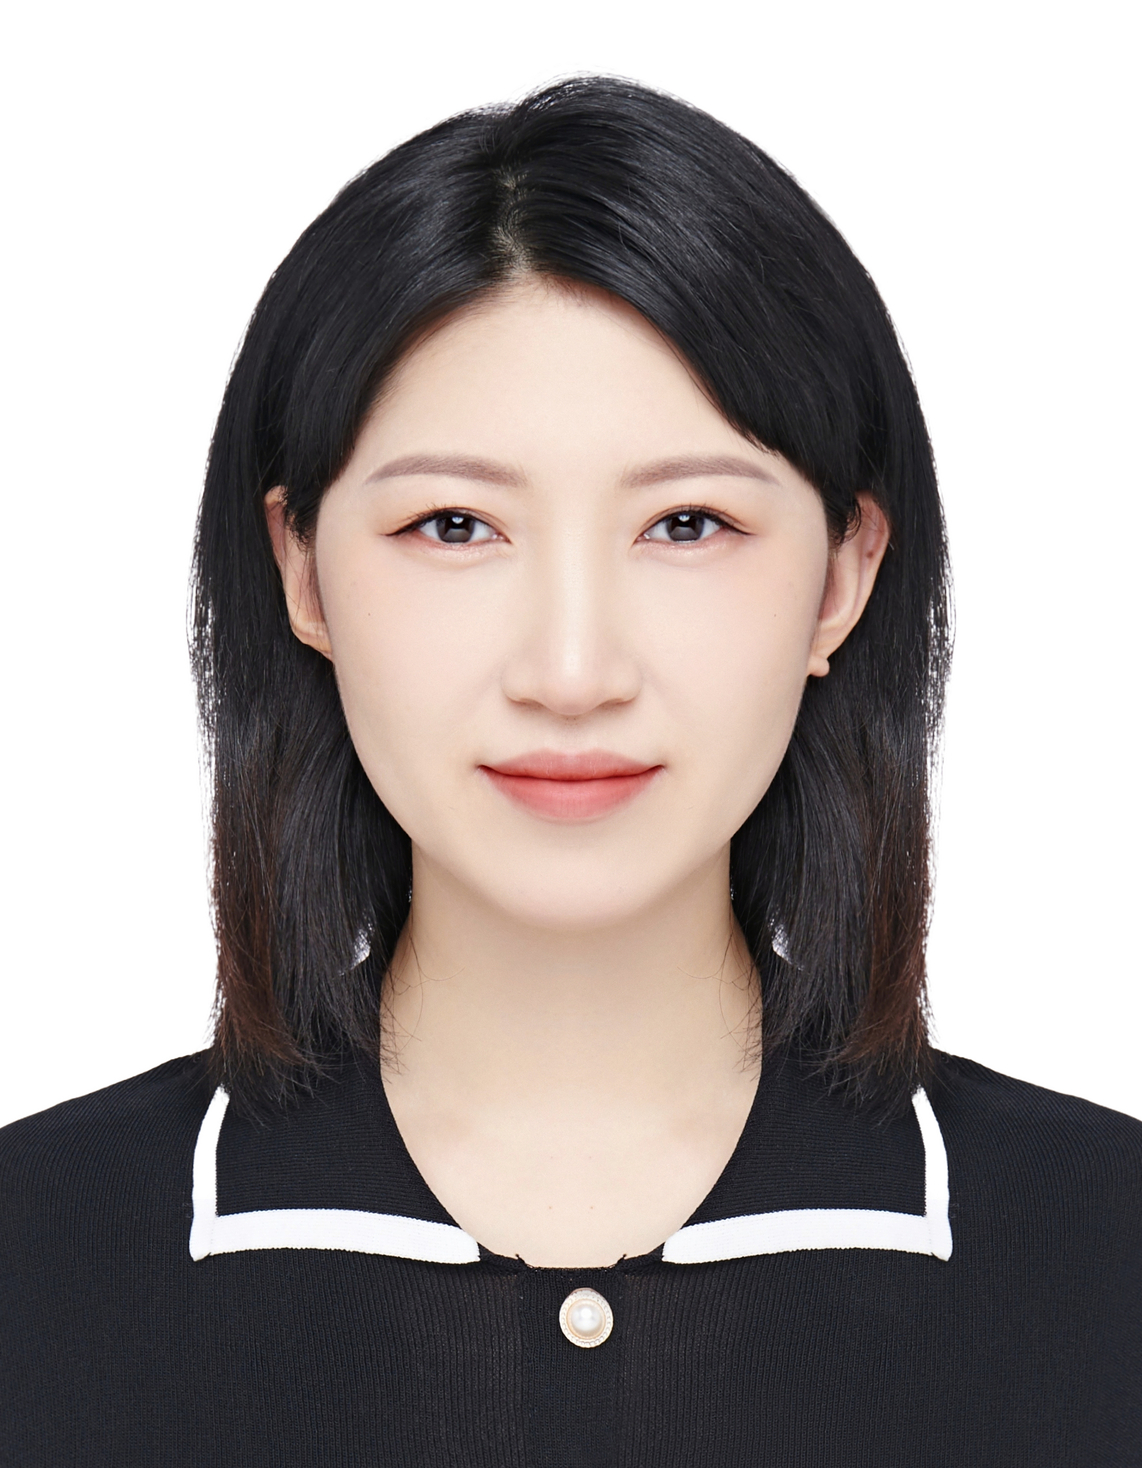
\includegraphics[width=0.9in,height=1.15in,clip,keepaspectratio]{author_figures/Liu_Dandan.jpg}}]{Dandan Liu} was born in China in 1991. She received the master's degree in journalism and communication from Fudan University, Shanghai, China. She is currently pursuing the Ph.D. degree with the Department of Media and Communication, Universiti Malaya, Kuala Lumpur, Malaysia. Her fields of study include crisis communication, health communication, and computer-mediated communication.
\end{IEEEbiography}

\begin{IEEEbiography}[{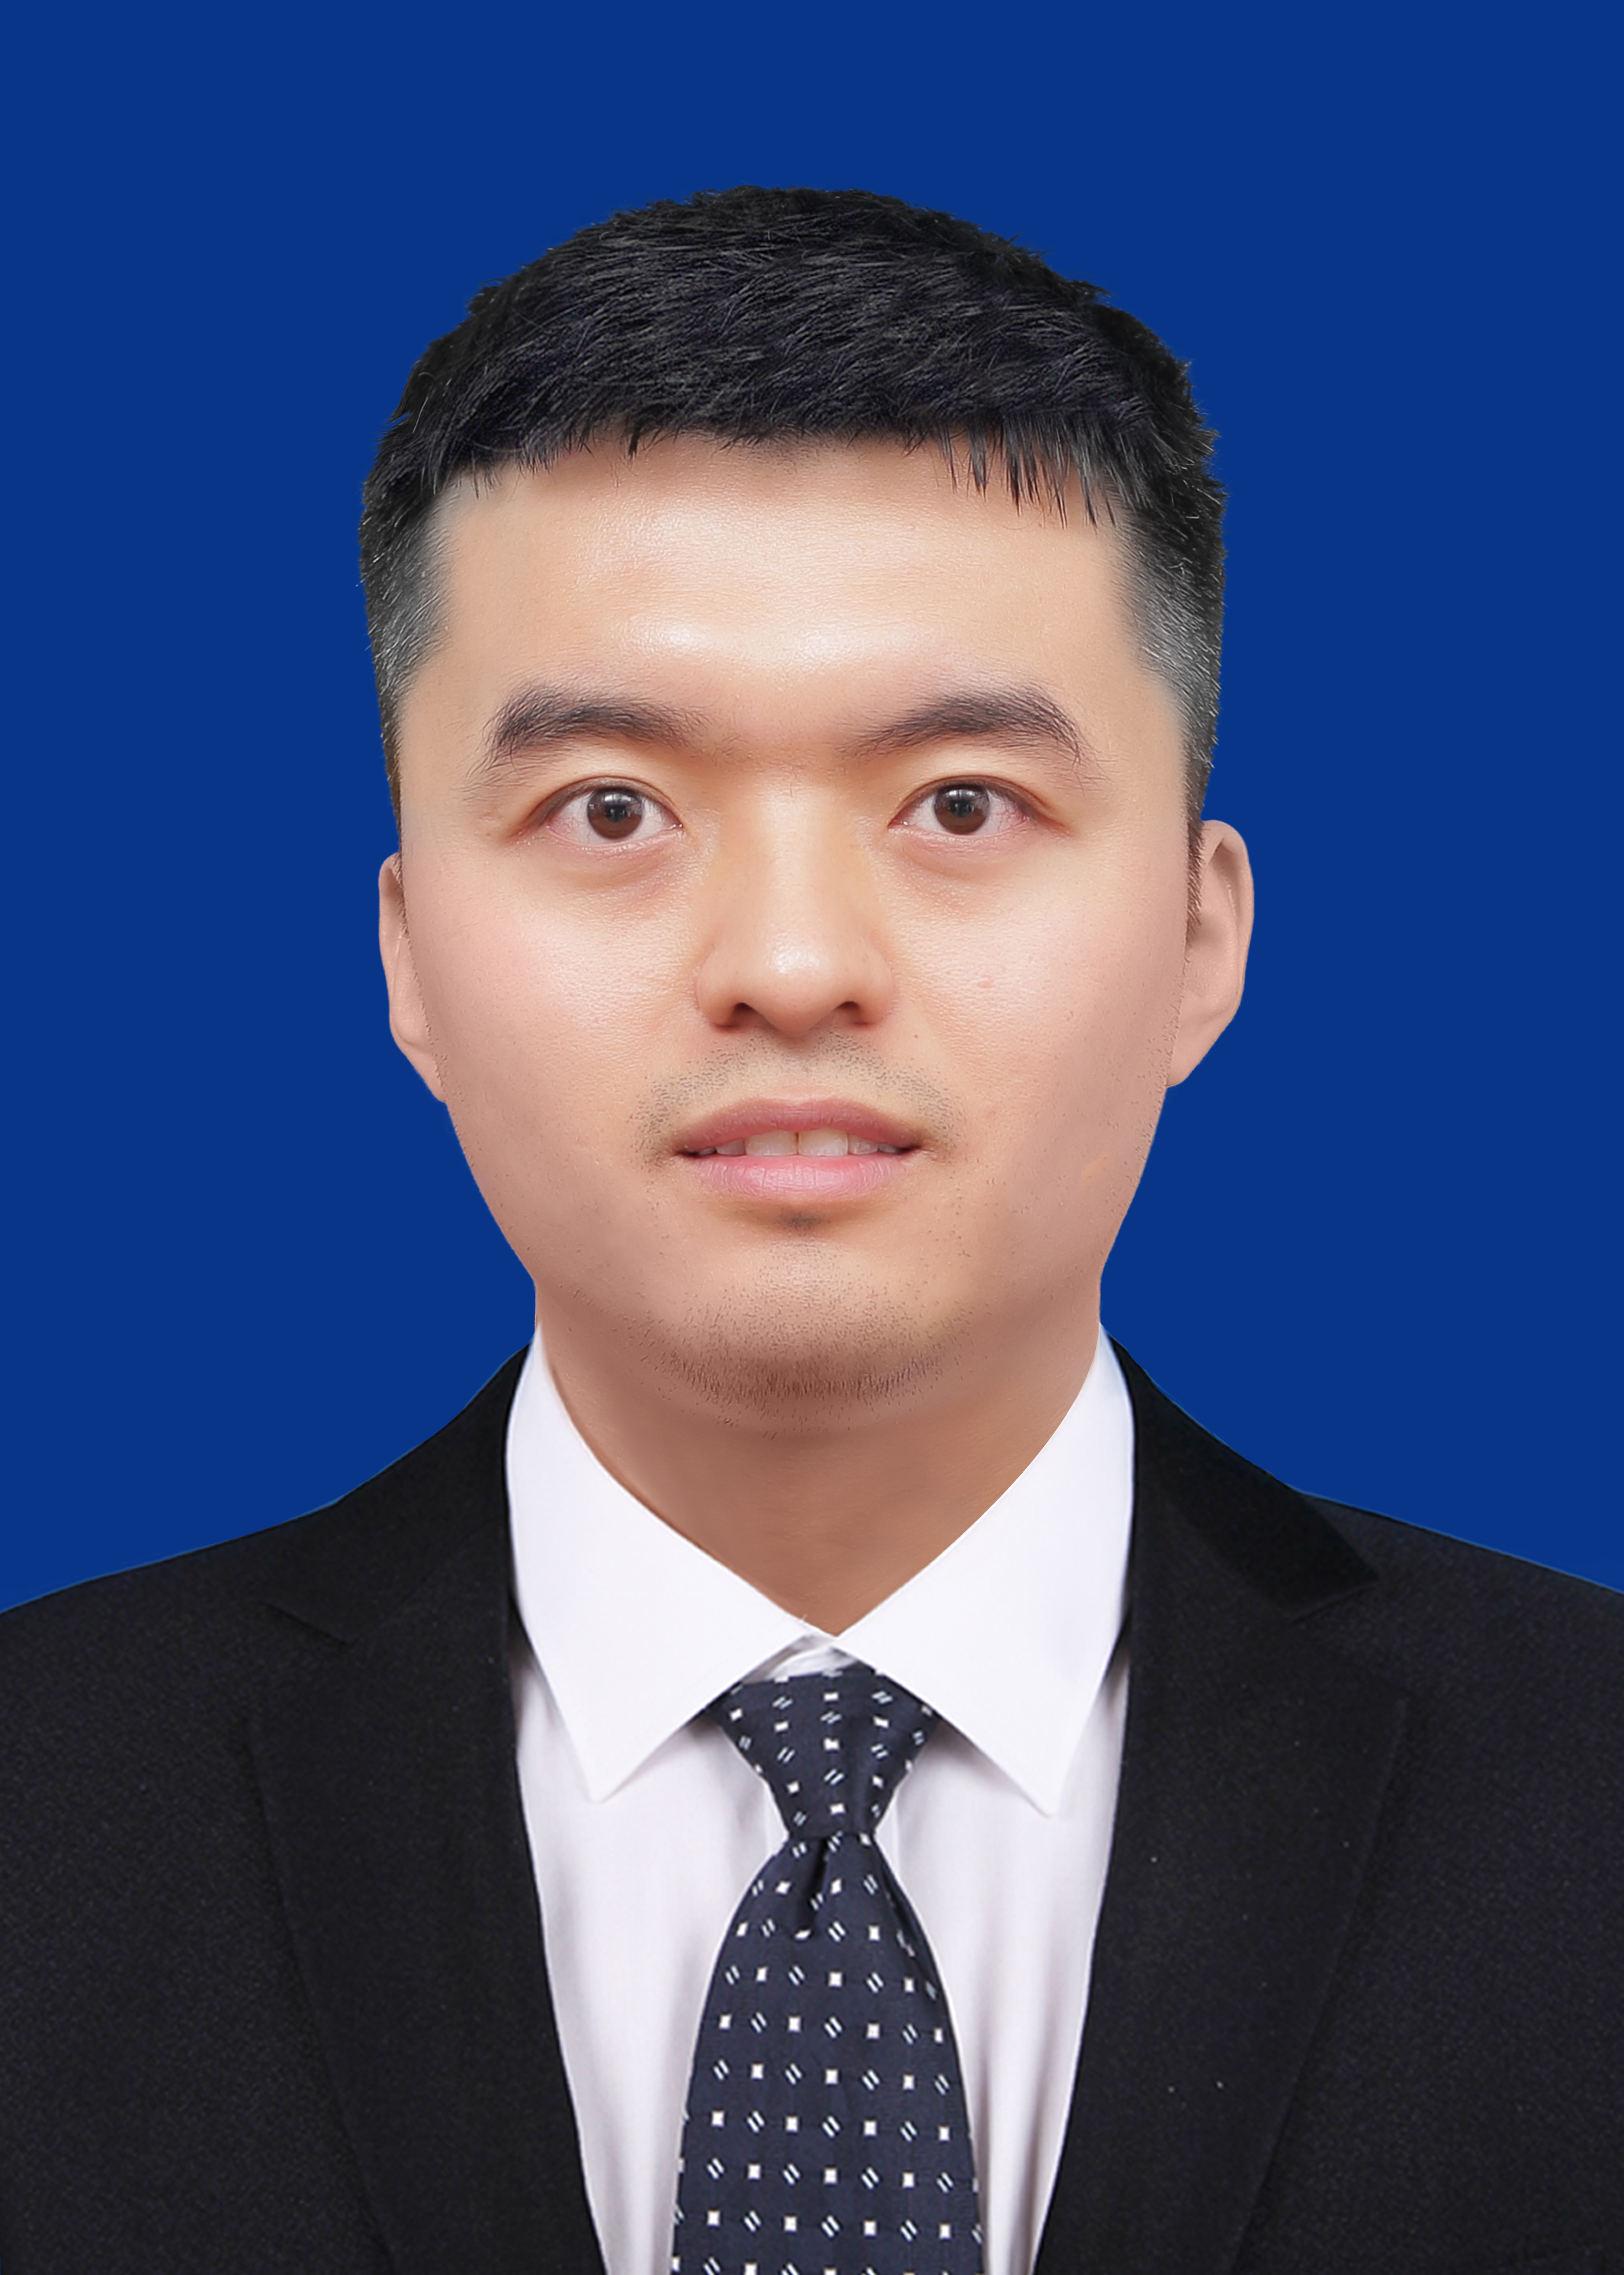
\includegraphics[width=0.9in,height=1.15in,clip,keepaspectratio]{author_figures/guangrui_fan.png}}]{Guangrui Fan} received the B.S. degree in digital media technology from Huazhong University of Science and Technology, Wuhan, China, in 2014, and the M.S. degree in software engineering from Shanghai Jiao Tong University, Shanghai, China, in 2018. He is currently pursuing the Ph.D. degree in computer science at Universiti Malaya, Kuala Lumpur, Malaysia. He is currently a lecturer at the School of Computer Science and Technology, Taiyuan University of Science and Technology, Taiyuan, China. His research focuses on human-centered artificial intelligence, human-AI interaction, AI in education and trust, social computing, algorithmic fairness. His work explores how AI systems can be designed, evaluated, and deployed in real-world learning, communication, online community, and social decision-making contexts. He has published more than 20 papers in his research fields, including CHI, ACL, ICML, WWW, AAAI, FSE, IJCAI, and IEEE Transactions journals. 
\end{IEEEbiography}

\begin{IEEEbiography}[{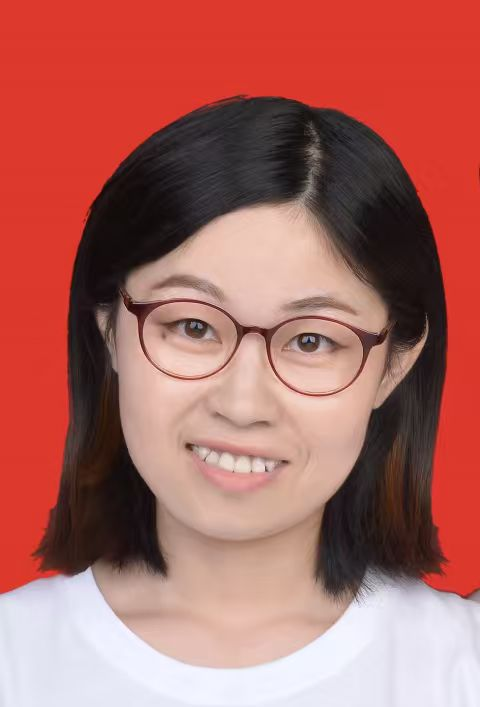
\includegraphics[width=0.9in,height=1.15in,clip,keepaspectratio]{author_figures/Guo_Qiang.jpg}}]{Qian Guo} received the M.S. and Ph.D. degrees in computer science and technology from Shanxi University, Taiyuan, China, in 2014 and 2022, respectively. She is currently an Associate Professor with the School of Computer Science and Technology, Taiyuan University of Science and Technology, Taiyuan, China. Her main research interests include multi-modal machine learning, logic learning, and their applications. She has published more than 20 papers in her research fields, including IEEE TPAMI, IEEE TEVC, ICML, and IJCAI.
\end{IEEEbiography}

\begin{IEEEbiography}[{
\includegraphics[width=0.9in,height=1.15in,clip,keepaspectratio]{author_figures/Zhang_Rui.jpg}}]{Rui Zhang} was born in Taiyuan, Shanxi Province, China, in February 1987. He is currently a Professor and Ph.D. Supervisor with the School of Computer Science and Technology, Taiyuan University of Science and Technology, Taiyuan, China. His primary research interests focus on intelligent information processing and related fields. His e-mail address is zhangrui@tyust.edu.cn.
\end{IEEEbiography}

\begin{IEEEbiography}[{\biophoto}]{Lihu Pan} received the Ph.D. degree. He is currently a Professor with Taiyuan University of Science and Technology, Taiyuan, China. His research interests include complex system simulation, deep learning, and software engineering. His e-mail address is panlh@tyust.edu.cn. Prof. Pan is a senior member of the Chinese Computer Society and a correspondent of the Software Engineering Committee of the Chinese Computer Society. He has presided over 20 scientific research projects, published 40 SCI/EI papers, authorized more than 10 invention patents, and received the second prize of the Provincial Science and Technology Progress Award.
\end{IEEEbiography}

\end{CJK*}
\end{document}


